\documentclass[11pt]{article}
\usepackage{amssymb,graphicx,amsmath,mathtools,float,subfig}
\usepackage{lscape}
\usepackage[utf8]{inputenc}
\usepackage[spanish, es-tabla]{babel}

\usepackage{indentfirst}	% Tabular tras un section
\usepackage{hyperref}
\hypersetup{
	colorlinks=false,
	citecolor=black,
	filecolor=black,
	linkcolor=red,
	urlcolor=black,
	pdfborderstyle={/S/U/W 1}
}

\usepackage[svgnames]{xcolor}
\definecolor{griscaption}{RGB}{100,100,100}
\usepackage{caption}
\usepackage[font={color=griscaption},figurename=Fig.,labelfont={bf}]{caption}


\newtheorem{theorem}{Teorema}
\newtheorem{corollary}[theorem]{Corolario}
\newtheorem{lemma}[theorem]{Lema}
\newtheorem{proposition}[theorem]{Proposición}
\newtheorem{definition}[theorem]{Definición}

\newcommand\ddfrac[2]{\frac{\displaystyle #1}{\displaystyle #2}}
\newcommand{\rulesep}{\unskip\ \vrule\ }






\title{Determinación de Órbitas Elípticas}
\author{Simón López
\\
{\small Matemáticas e Ingeniería Informática}
\\
{\small Universidad de Granada, 18071 Granada, Spain}
\\
{\small simondelosbros@correo.ugr.es}}
\date{\today}
\setlength{\unitlength}{1cm}
\setlength{\unitlength}{1cm}


\begin{document}


\section{Método Laplaciano de Determinación}
%Determinar el valor de la primera y segunda derivada de $\lambda$, $\mu$, $\nu$, $X$, $Y$, $Z$ en algún momento $t$.
\subsection{\normalfont{\textit{Determinación de las derivadas de $\lambda$, $\mu$, $\nu$ en algún momento $t$.}}}
\label{subsec:primera_segunda_derivada}
Dado que no podemos calcular el valor exacto de las derivadas de $\lambda$, $\mu$, $\nu$, utilizaremos fórmulas de derivación numérica con dos nodos para obtener un valor aproximado de éstas. Tomemos, por ejemplo, $t=t_2$, que por el momento nos bastará para demostrar que se puede realizar una buena aproximación. Supongamos que el valor de $\lambda'$ no cambia muy rápido; entonces, el valor de la derivada en $t_2$ en el intervalo $[t_1,t_2]$ será muy cercano al valor de:
\[
\lambda_{12}'=\frac{\lambda(t_2)-\lambda(t_1)}{t_2-t_1},
\]

\noindent y dado que los nodos elegidos cumplen $t_2>t_1$, estaremos ante una diferencia regresiva. Análogamente podremos aproximar el valor de la derivada en $t_2$ mediante una diferencia progresiva, a la que llamaremos $\lambda_{23}'$.\\

El error de estas aproximaciones, suponiendo que $\lambda$ sea de clase 2 en el intervalo de aproximación, es del orden de $(t_2-t_1)$ y $(t_3-t_2)$ para $\lambda_{12}'$ y $\lambda_{23}'$ respectivamente. Por tanto, cuanto más pequeño sea el intervalo donde realizamos las operaciones, es de esperar que la aproximación obtenida sea mejor. Además, si la longitud del intervalo $[t_1,t_2]$ es igual a la longitud de $[t_2,t_3]$, podremos calcular el valor aproximado de $\lambda'$ en $t_2$ mediante una diferencia centrada, obteniendo:
\[
\lambda'_2=\frac{\lambda_{12}'+\lambda_{23}'}{2}
\]

Si los intervalos tienen una longitud diferente, podremos ajustar la disparidad entre ellos para realizar la aproximación o utilizar un método diferente para aproximar la derivada, como veremos en \ref{subsec:series_potencias}.\\

Análogamente podremos definir la derivada segunda de $\lambda$ en $t_2$, en la que utilizaremos los valores de la primera derivada obtenidos anteriormente:
\[
\lambda''_2=\frac{\lambda_{23}'-\lambda_{12}'}{\frac{1}{2}(t_3-t_1)}
\]

Dicha aproximación será de orden $(t_3-t_1)^2$ siempre que $\lambda\in\mathcal{C}^4[t_1,t_3]$. Mediante este mismo método calcularemos la primera y segunda derivada de $\mu$ y $\nu$; además, podemos suponer que las tres funciones son de clase infinito en todo $\mathbb{R}$.\\

Como hemos comentado antes, las aproximaciones obtenidas de esta manera es razonable que sean más cercanas cuanto menor sea la longitud de los intervalos entre las observaciones, y generalmente, en la práctica, los intervalos que utilizaremos serán cortos.\\

Finalmente, necesitaremos tener los valores de la primera y segunda derivada de $X$, $Y$, $Z$, correspondientes al vector de $S$ a $E$, aunque no tendremos por qué calcularlos de manera aproximada. Para obtener dichas cantidades exactas utilizaremos la efemérides proporcionada por el \href{https://ssd.jpl.nasa.gov/horizons.cgi}{\textit{Jet Propulsion Laboratory}} en su página web, que nos dará el valor de estas variables para cualquier día del año, a cualquier hora y desde cualquier coordenada terrestre. Notar que aquí solo aparecerá la posición y velocidad, pero dado que $E$ gira alrededor de $S$ en concordancia con la ley de Gravitación Universal, podremos calcular la segunda derivada mediante:
\begin{align}
\left\{
\def\arraystretch{2}
\begin{array}{l}
	X'' = -\ddfrac{k^2X}{R^3}\\
	Y'' = -\ddfrac{k^2Y}{R^3}\\
	Z'' = -\ddfrac{k^2Z}{R^3}
\end{array}
\right.
\label{eq:ley_gravitacion_S_E}
\end{align}

\noindent donde $k^2=GM$, parámetro gravitacional estándar, $G=6.674\times10^{-11}\frac{\text{N}\cdot\text{m}^2}{\text{kg}^2}$ constante de gravitación y $M=1.989\times10^{30}\;\text{kg}$ masa del Sol. Tomamos solo la masa del Sol, $M$, ya que la masa de nuestro cuerpo es despreciable en comparación con ésta usando como modelo el problema de Kepler.\\



%Imponer la condición de que $C$ gira en torno a $S$ de acuerdo a la ley de gravitación.
\subsection{\normalfont{\textit{Imponer la condición de que $C$ gira en torno a $S$ de acuerdo a la ley de gravitación.}}}
\label{subsec:ley_gravitacion}
Asumiendo que el cuerpo observado $C$ no está alterado por la interacción con otros cuerpos cercanos, podemos asegurar que cumplirá el problema de Kepler, dando lugar a las siguientes ecuaciones diferenciales:
\begin{align}
\left\{
\def\arraystretch{2}
\begin{array}{l}
	\ddfrac{d^2x}{dt^2}=-\ddfrac{k^2x}{r^3}\\
	\ddfrac{d^2y}{dt^2}=-\ddfrac{k^2y}{r^3}\\
	\ddfrac{d^2z}{dt^2}=-\ddfrac{k^2z}{r^3}
\end{array}
\right.
\label{eq:ley_gravitacion_S_C}
\end{align}

\noindent análogas a las que hemos visto para $S$ y $E$ en \eqref{eq:ley_gravitacion_S_E}.\\

Además, utilizando las \hyperref[eq:terminologia]{relaciones entre $E$, $C$ y $S$}, así como los resultados vistos anteriormente, llegamos a:
\begin{align}
\left\{
\begin{array}{l}
	x=\rho\lambda-X\\
	y=\rho\mu-Y\\
	z=\rho\nu-Z
\end{array}
\right.
\label{eq:relacion_C_S_E}
\end{align}

\noindent y sustituyendo los valores obtenidos en las  ecuaciones \eqref{eq:ley_gravitacion_S_C}, obtenemos:
\begin{align}
\left\{
\def\arraystretch{2}
\begin{array}{l}
	(\rho\lambda)'' - X'' = \ddfrac{-k^2(\rho\lambda-X)}{r^3}\\
	(\rho\mu)'' - Y'' = \ddfrac{-k^2(\rho\mu-Y)}{r^3}\\
	(\rho\nu)'' - Z'' = \ddfrac{-k^2(\rho\nu-Z)}{r^3}
\end{array}
\right.
\label{eq:derivada_segunda}
\end{align}

Desarrollando la segunda derivada de $\rho\lambda$ llegamos a:
\[
(\rho\lambda)''=(\rho'\lambda+\rho\lambda')'=\rho''\lambda+2\rho'\lambda'+\rho\lambda'',
\]

\noindent valor que utilizaremos más adelante.\\

Utilizando el resultado \eqref{eq:ley_gravitacion_S_E}, sustituyendo en la ecuación \eqref{eq:derivada_segunda} y desarrollando llegamos a lo siguiente:
\begin{align}
\left\{
\def\arraystretch{2}
\begin{array}{l}
	\lambda\rho''+2\lambda'\rho'+[\lambda''+\ddfrac{k^2\lambda}{r^3}]\rho=-k^2X[\ddfrac{1}{R^3}-\ddfrac{1}{r^3}]\\
	\mu\rho''+2\mu'\rho'+[\mu''+\ddfrac{k^2\mu}{r^3}]\rho=-k^2Y[\ddfrac{1}{R^3}-\ddfrac{1}{r^3}]\\
	\nu\rho''+2\nu'\rho'+[\nu''+\ddfrac{k^2\nu}{r^3}]\rho=-k^2Z[\ddfrac{1}{R^3}-\ddfrac{1}{r^3}]
\end{array}
\right.
\label{eq:fundamental_equations}
\end{align}

\noindent a las que llamaremos ecuaciones fundamentales. Así, las incógnitas de las ecuaciones a resolver pasan a ser $r, \; \rho, \; \rho'$ y $\rho''$.\\



\subsection{\normalfont{\textit{Determinación de las distancias de $C$ a $E$ y $S$.}}}
\label{subsec:distancias}
Actualmente disponemos de un vector unitario $(\lambda,\mu,\nu)$ que apunta desde la Tierra hacia el cuerpo observado, pero desconocemos la distancia que hay entre estos dos cuerpos. Para determinar tanto esta distancia como la que hay desde $S$ hasta $C$, utilizaremos las ecuaciones fundamentales obtenidas al final del paso anterior, \eqref{eq:fundamental_equations}, y una condición geométrica que cumplirán los tres cuerpos. Para llevar a cabo esto, tomaremos el sistema \eqref{eq:fundamental_equations} como un sistema lineal en $\rho$, $\rho'$ y $\rho''$ y resolveremos utilizando la regla de Cramer. Comencemos definiendo el siguiente determinante:
\[
D =
\left|
\begin{array}{ccc}
	\lambda & 2\lambda' & \lambda''+\frac{k^2\lambda}{r^3}\\
	\mu & 2\mu' & \mu''+\frac{k^2\mu}{r^3}\\
	\nu & 2\nu' & \nu''+\frac{k^2\nu}{r^3}
\end{array}
\right|
=
2
\left|
\begin{array}{ccc}
	\lambda & \lambda' & \lambda''\\
	\mu & \mu' & \mu''\\
	\nu & \nu' & \nu''
\end{array}
\right|
=2W(\lambda,\mu,\nu)
\]

\noindent siendo $W(\lambda,\mu,\nu)$ el Wronskiano de las coordenadas angulares. La segunda forma del determinante ha sido obtenida mediante la transformación $C_3-\frac{k^2\lambda}{r^3}C_1$ sobre la matriz, donde $C_i$ representará la columna i-ésima. Una vez hayamos sustituido las derivadas exactas por su valor aproximado calculado anteriormente, conoceremos todas las cantidades de este determinante.\\

Por otra parte, definiremos el determinante $D_1$, que utilizaremos para calcular $\rho$ mediante la regla de Cramer, reemplazando la tercera columna por los términos independientes del sistema \eqref{eq:fundamental_equations} y omitiendo el factor $[\frac{1}{R^3}-\frac{1}{r^3}]$, que añadiremos más adelante. De nuevo, conocemos todas las cantidades utilizadas. Así, obtenemos el siguiente determinante:
\[
D_1 = -2k^2
\left|
\begin{array}{ccc}
\lambda & \lambda' & X\\
\mu & \mu' & Y\\
\nu & \nu' & Z
\end{array}
\right|
\]

Con todo esto, la distancia $\rho$ será determinada por:
\[
\rho = \frac{D_1}{D}[\frac{1}{R^3}-\frac{1}{r^3}],
\]

El valor de $r$ es desconocido, por lo que añadiremos la siguiente ecuación formando con la anterior un sistema de ecuaciones en $r$ y $\rho$.
\begin{align}
r^2=\rho^2+R^2-2\rho R\cos\psi,
\label{eq:triangle_relations_1}
\end{align}

\noindent donde $\psi$ es el ángulo formado en $E$ trazando una línea imaginaria hasta el Sol y hasta el cuerpo observado, es decir, entre $R$ y $\rho$; esta ecuación expresa el hecho de que $S$, $E$ y $C$ forman un triángulo como vimos en la \hyperref[figure:1]{figura 1}.\\

Dado que disponemos de los valores $\overrightarrow{SE}=(X,Y,Z)$ y $\overrightarrow{EC}=(\lambda,\mu,\nu)$, vector unitario, podremos obtener el coseno de $\psi$ con:
\[
\cos{\psi}=\frac{\langle\overrightarrow{SE},\overrightarrow{EC}\rangle}{|\overrightarrow{SE}||\overrightarrow{EC}|}=\frac{\langle(X,Y,Z),(\lambda,\mu,\nu)\rangle}{R}
\]

Resolviendo el sistema de ecuaciones al que hemos llegado obtendremos los valores de $\rho$ y $r$, habiendo terminado este paso. Más adelante discutiremos la unicidad de la solución en el sistema con $r,\rho>0$ (\ref{subsec:unicidad}). Al encontrar la solución de este sistema podremos calcular las coordenadas de $C$ mediante las ecuaciones \eqref{eq:relacion_C_S_E} de las relaciones entre $S$, $E$ y $C$.\\

\subsection{\normalfont{\textit{Determinación de las componentes de velocidad de $C$.}}}
\label{subsec:velocity_component}
Se sigue de las ecuaciones \eqref{eq:relacion_C_S_E} que:
\[
\left\{
\begin{array}{l}
	x'=\rho'\lambda+\rho\lambda'-X'\\
	y'=\rho'\mu+\rho\mu'-Y'\\
	z'=\rho'\nu+\rho\nu'-Z'
\end{array}
\right.	
\]

En estas ecuaciones solo tenemos una incógnita, $\rho'$, que podremos determinar resolviendo por Cramer en \eqref{eq:fundamental_equations} a partir de:
\[
\rho'=+\frac{D_2}{D}[\frac{1}{R^3}-\frac{1}{r^3}],
\; \; \; \; \; \; \; \; \; \text{ con } \;
D_2 = -k^2
\left|
\begin{array}{ccc}
\lambda & X & \lambda''\\
\mu & Y & \mu''\\
\nu & Z & \nu''
\end{array}
\right|
\]

Notar que en $D_2$ también hemos realizado la operación $C_3-\frac{k^2\lambda}{r^3}C_1$, como en $D$, para obtener un determinante más simple.\\

Dado que ya conocemos el valor de $r$ podremos calcular directamente $\rho'$, y de esta manera $x'$, $y'$ y $z'$ se vuelven conocidas.\\

\subsection{\normalfont{\textit{Determinación de los elementos orbitales a partir de la posición y velocidad del cuerpo observado.}}}
\label{subsec:elements_determination}
Una vez conocida tanto la posición como la velocidad del cuerpo en un instante determinado, nos dispondremos a calcular los elementos orbitales mediante las distintas fórmulas estudiadas en el manual de Mecánica Celeste\cite{ortega}. Denotemos por $r(t)=(x,y,z)(t)$ la posición del objeto y $v(t)$ su derivada, la velocidad.\\

Comencemos determinando la energía que tiene nuestro cuerpo en un instante $t$. Para ello utilizaremos:
\[
h=\frac{|v(t)|^2}{2}-\frac{\mu}{|r(t)|}
\]

\noindent donde $\mu=GM$ una constante positiva. Con el valor de la energía podemos pasar a calcular la primera de nuestros elementos astronómicos, la longitud del semieje mayor, $a$, utilizando la siguiente ecuación:
\[
a=-\frac{\mu}{2h}
\]

Pasemos ahora a calcular el momento angular de nuestro objeto. Dado que la masa del objeto observado es despreciable frente a la masa del Sol, podremos obviar su valor, obteniendo así el vector del momento angular mediante:
\[
c=r(t)\wedge v(t)
\]

Calculado el momento angular, podremos obtener el vector de excentricidad para la órbita del cuerpo observado:
\[
\vec{e}=-\frac{r(t)}{|r(t)|}-\frac{1}{\mu}(c\wedge v(t))
\]

\noindent y la excentricidad de la órbita será $e=|\vec{e}|$.\\

Una vez obtenidos estos valores, podemos utilizaremos la tercera ley de Kepler para obtener el período mínimo (suponiendo que nuestra órbita se corresponda con la de una elipse). Si el momento angular del objeto observado $c\neq0$ y su energía $h<0$, entonces la órbita es periódica y su período mínimo valdrá:
\[
p=\frac{2\pi}{\sqrt{\mu}}a^{3/2}
\]

Sabemos que el vector del momento angular, del que disponemos, es el vector normal al plano orientado de la órbita, pudiendo calcular así la inclinación del plano de movimiento. Además, calculando la intersección de éste con el plano de la eclíptica obtenemos la línea de nodos y con ella el nodo ascendente $\mathcal{N}_+$, con la que podremos determinar $\Omega$.
\[
\left\{
\begin{array}{l}
	i=\measuredangle(\vec{e}_3,\vec{n}), \; \; \; \; \; \; \; \; \; \; i\in]0,\pi[\\
	\Omega=\measuredangle(\vec{e}_1, \mathcal{N}_+), \; \; \; \; \; \Omega\in\mathbb{R}/2\pi\mathbb{Z}
\end{array}
\right.
\]

Finalmente usaremos el vector de excentricidad $\vec{e}$ para calcular $\omega$, utilizando el nodo ascendente como eje de rotación.\\


\subsection{\normalfont{\textit{Determinación de las derivadas de $\lambda$, $\mu$, $\nu$ mediante interpolación.}}}
\label{subsec:series_potencias}
Tal y como hemos visto en la sección \ref{subsec:primera_segunda_derivada}, hemos de calcular la primera y segunda derivada de las coordenadas angulares $\lambda$, $\mu$, $\nu$. El problema es que no siempre los intervalos de tiempo en los que hacemos la medida del objeto en el cielo son equiespaciados, y por tanto no podremos obtener una aproximación mediante diferencias centradas. Por tanto, busquemos un nuevo método para obtener las derivadas aproximadas de nuestras coordenadas angulares.\\

Comencemos recordando las ecuaciones \eqref{eq:ley_gravitacion_S_C}:
\begin{align}
\left\{
\def\arraystretch{2}
\begin{array}{l}
	\ddfrac{d^2x}{dt^2}=-\ddfrac{k^2x}{r^3}\\
	\ddfrac{d^2y}{dt^2}=-\ddfrac{k^2y}{r^3}\\
	\ddfrac{d^2z}{dt^2}=-\ddfrac{k^2z}{r^3}
\end{array}
\right.
\label{eq:ley_gravitacion_C_2}
\end{align}

La solución para estas ecuaciones diferenciales de segundo orden puede ser expandida como serie de Taylor en $t$, y esta convergerá siempre que el valor de $t$ no sea especialmente grande.
\begin{align}
\left\{
\def\arraystretch{2}
\begin{array}{l}
	x=x_0+x_0't+\ddfrac{1}{2}(\ddfrac{d^2x}{dt^2})_0t^2+...+\ddfrac{1}{n!}(\ddfrac{d^nx}{dt^n})_0t^n+...\\
	y=y_0+y_0't+\ddfrac{1}{2}(\ddfrac{d^2y}{dt^2})_0t^2+...+\ddfrac{1}{n!}(\ddfrac{d^ny}{dt^n})_0t^n+...\\
	z=z_0+z_0't+\ddfrac{1}{2}(\ddfrac{d^2z}{dt^2})_0t^2+...+\ddfrac{1}{n!}(\ddfrac{d^nz}{dt^n})_0t^n+...\\	
\end{array}
\right.
\label{eq:series_taylor}
\end{align}

En las ecuaciones superiores el subíndice 0 indicará que tomamos el valor $t=0$ en la función. Podemos sustituir la segunda derivada que aparece en estas series por su valor en \eqref{eq:ley_gravitacion_C_2}, la tercera derivada por la derivada de ésta y a partir de la cuarta derivada repetimos este proceso, teniendo así que las series estarán solo en función de la $x$, $y$, $z$ y la primera derivada de cada una de estas, todos ellas tomadas en $t=0$.\\

Los tres valores $x$, $y$, $z$, a los que en conjunto llamaremos $r(t)$, forman una solución del problema de Kepler. Además, sabemos que la fórmula de las soluciones para el problema de Kepler es:
\[
r(t)=a(\cos{u(t)}-e,\sqrt{1-e^2}\sin{u(t)})
\]

\noindent donde $u(t)$ es la anomalía. Dado que la ecuación está formada por funciones trigonométricas, que son analíticas, y la anomalía es una función analítica por el teorema de la función implícita, llegamos a que $r(t)$ será también una función analítica.\\

Hemos de tener en cuenta que el valor de estas series no siempre tiene valor práctico, pues el intervalo de tiempo para la convergencia puede ser demasiado grande; notar que los límites serán más pequeños cuanto más pequeña sea la distancia del perihelio y más grande la excentricidad de nuestra órbita.\\

En el caso de la Tierra, expandiendo sus coordenadas en series de potencias, obtendremos una convergencia durante largos intervalos de tiempo debido a la pequeña excentricidad de la órbita terrestre ($e\approx0.0167$). Así, se sigue de la ecuación \eqref{eq:relacion_C_S_E}, que relaciona las coordenadas de la Tierra, el Sol y el cuerpo observado que las ecuaciones de $\rho$, $\lambda$, $\mu$, $\nu$ también son funciones analíticas y por ello podrán ser expandidas como series de Taylor, con el mismo rango de utilidad que el de las series para $x$, $y$ y $z$.\\

Veamos las series para $\lambda$, pues las de $\mu$ y $\nu$ serán simétricamente similares. Tomando los valores $t_1$, $t_2$ y $t_3$, las series para $\lambda$ serán:
\begin{align}
\left\{
\begin{array}{l}
	\lambda(t)=c_0+c_1t+c_2t^2+...\\
	\lambda(t_1)=c_0+c_1t_1+c_2t_1^2+...\\
	\lambda(t_2)=c_0+c_1t_2+c_2t_2^2+...\\
	\lambda(t_3)=c_0+c_1t_3+c_2t_3^2+...
\end{array}
\right.
\label{eq:series_lambda}
\end{align}

\noindent donde los valores $c_0, c_1, c_2, ...$ son constantes. Si estas series terminan tras los términos elevados al cuadrado, podremos determinar $c_0$, $c_1$ y $c_2$ resolviendo como un sistema de ecuaciones, ya que conocemos las cantidades $\lambda(t_1)$, $\lambda(t_2)$, $\lambda(t_3)$. Así, tenemos que cuantas más observaciones tengamos disponibles, más coeficientes podrán ser determinados.\\

Tomamos ahora el sistema de ecuaciones \eqref{eq:series_lambda}; si queremos que sea compatible, su determinante ha de ser 0, pues tenemos tres incógnitas y cuatro ecuaciones, es decir, nos ``sobra'' una ecuación (sistema compatible indeterminado). Así, podemos obtener la siguiente igualdad:
\begin{align}
\left|
\begin{array}{cccc}
\lambda(t)   & 1 & t   & t^2  \\
\lambda(t_1) & 1 & t_1 & t^2_1\\
\lambda(t_2) & 1 & t_2 & t^2_2\\
\lambda(t_3) & 1 & t_3 & t^2_3\\
\end{array}
\right|
=0
\label{eq:resultante}
\end{align}

Si resolvemos este determinante desarrollando por la primera columna y despejamos $\lambda$ obtenemos:
\begin{align}
\lambda(t)_L=
\frac{(t-t_2)(t-t_3)}{(t_1-t_2)(t_1-t_3)}\lambda(t_1)
+\frac{(t-t_3)(t-t_1)}{(t_2-t_3)(t_2-t_1)}\lambda(t_2)
+\frac{(t-t_1)(t-t_2)}{(t_3-t_1)(t_3-t_2)}\lambda(t_3)
\label{eq:lambda_value}
\end{align}

Utilizamos el subíndice $L$ para denotar que esta función es aproximada y no proporcionará el valor exacto de $\lambda$ (salvo en ciertos casos).\\

Dicho polinomio corresponderá al polinomio de interpolación de Lagrange con el que obtendremos un valor aproximado de $\lambda$. Hemos de tener en cuenta que los valores en los nodos $t_1$, $t_2$, $t_3$ han de ser diferentes entre sí para que no se anulen los denominadores.\\

Con esto, somos capaces de obtener $\lambda$ de manera exacta en $t_1$, $t_2$ y $t_3$; para otros valores diferentes de $t$ obtendremos $\lambda$ de forma aproximada. Para obtener un valor exacto de $\lambda$ habremos de tomar la primera ecuación de \eqref{eq:series_lambda}, una serie infinita, dentro de su rango de convergencia.\\

Como comentamos anteriormente, el polinomio de interpolación de Lagrange obtenido nos proporcionará valores aproximados de $\lambda$, por lo que será conveniente estudiar el error de éste, que tomando la primera ecuación de \eqref{eq:series_lambda} será:
\[
|\lambda(t)-\lambda_L(t)|
\]

Dado que en anteriores secciones hemos supuesto que $\lambda$, $\mu$, $\nu$ son de clase infinito, podemos aplicar el teorema de error de interpolación, que nos dará una fórmula para obtener el error para todo $t$. Utilizando los tres nodos $t_1$, $t_2$, $t_3$ obtenemos:
\begin{align}
\lambda(t)-\lambda_L(t)=\ddfrac{\lambda^{\romannumeral 4}(\xi)}{4!}(t-t_1)(t-t_2)(t-t_3)
\label{eq:interpolation_error}
\end{align}

\noindent donde $\min{(t,t_1,t_2,t_3)}<\xi<\max{(t,t_1,t_2,t_3)}$. El cálculo de $\xi$ es complicado, pero podremos tomar una cota superior para $\lambda^{\romannumeral 4}$. Sea $K_4$ dicha cota, con $|\lambda^{\romannumeral 4}(x)|\leq K_4$, entonces el error de la interpolación será:
\begin{align}
|\lambda(t)-\lambda_L(t)|\leq\ddfrac{K_4}{4!}(t-t_1)(t-t_2)(t-t_3)
\label{eq:interpolation_error_cota}
\end{align}

Utilizando un mayor número de observaciones dispondremos de más nodos; así, si hemos realizado $N$ observaciones, la ecuación para el error será:
\begin{align}
|\lambda(t)-\lambda_L(t)|\leq\ddfrac{K_N}{(N+1)!}(t-t_1)...(t-t_N)
\label{eq:interpolation_error_n_observations}
\end{align}


%%%
%Considerando esta serie geométricamente podemos definir una curva que llamaremos $C$; por otra parte definiremos la curva $C_2$ como la que produce el polinomio de interpolación \eqref{eq:lambda_value}. Representando las dos en una misma gráfica podemos visualizar la diferencia entre el valor real y el aproximado mediante interpolación de las funciones estudiadas:
%\begin{figure}[H]
%\centering
%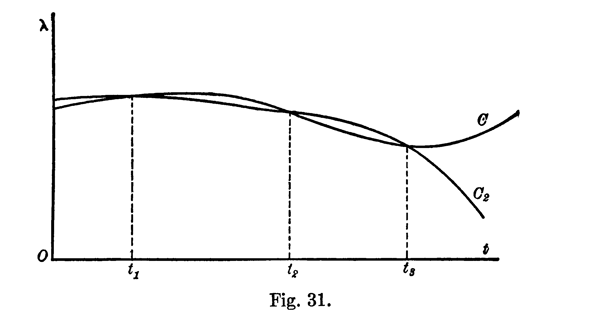
\includegraphics[scale=0.5]{images/fig_31.png}
%\end{figure}
%Dichas curvas se intersecan en $\tau_1$, $\tau_2$ y $\tau_3$, y en general en ningún otro punto; tomando valores pequeños de $\tau$ las dos curvas casi coincidirán.\\
%%%


Con el estudio del error y todo lo visto anteriormente, podemos justificar que la diferencia entre los valores de $t$ ha de ser pequeña en la práctica para que las cantidades aproximadas calculadas sean lo más cercanas a su valor original. Además, no tendría sentido una diferencia de tiempo muy grande entre las observaciones del objeto, pues pasaríamos mucho tiempo para determinar una única órbita.\\

Por último, ya que necesitamos la primera y segunda derivada de $\lambda$, nos bastará con derivar del polinomio \eqref{eq:lambda_value}.
\begin{align*}
\lambda'(t)_L = \frac{2t-(t_2+t_3)}{(t_1-t_2)(t_1-t_3)}\lambda(t_1)
+\frac{2t-(t_3+t_1)}{(t_2-t_3)(t_2-t_1)}\lambda(t_2)
+\frac{2t-(t_1+t_2)}{(t_3-t_1)(t_3-t_2)}\lambda(t_3)\\
\lambda''(t)_L = \frac{2}{(t_1-t_2)(t_1-t_3)}\lambda(t_1)
+\frac{2}{(t_2-t_3)(t_2-t_1)}\lambda(t_2)
+\frac{2}{(t_3-t_1)(t_3-t_2)}\lambda(t_3)
\end{align*}

Tal y como comentamos anteriormente, se procederá al cálculo de $\mu$ y $\nu$ y al estudio de su error de aproximación de manera similar a la desarrollada en este apartado.

\newpage


\section{Estudio del número de soluciones admisibles}

\subsection{\normalfont{\textit{Ecuaciones fundamentales en el método de Laplace.}}}
\label{subsec:fundamental_equations}
Para terminar la explicación del método de determinación con tres observaciones, recapitulemos viendo las principales ecuaciones utilizadas para obtener la órbita del objeto observado. Las ecuaciones fundamentales serán las de \eqref{eq:fundamental_equations}, que involucrarán las coordenadas angulares $\lambda$, $\mu$, $\nu$ y sus derivadas, las cuáles conocemos su valor aproximado por \ref{subsec:primera_segunda_derivada} o \ref{subsec:series_potencias}. Por otra parte, el valor de $\rho$ y sus derivadas se obtendrá resolviendo las ecuaciones fundamentales utilizando la regla de Cramer, como vimos en anteriores apartados, aunque discutiremos más adelante otro método para su cálculo.\\

Hasta ahora disponemos de $\rho$ y $\rho'$; nos faltaría por calcular $\rho''$. Comencemos definiendo el determinante $D_3$:
\[
D_3=-2k^2
\left|
\begin{array}{ccc}
X & \lambda' & \lambda''\\
Y & \mu' & \mu''\\
Z & \nu' & \nu''
\end{array}
\right|
\]

Tras ello, calculemos el determinante $D$ cambiando la primera columna por el término independiente de \eqref{eq:fundamental_equations}, sin tomar $[\frac{1}{R^3}-\frac{1}{r^3}]$. 
\[
\left|
\begin{array}{ccc}
-k^2X & 2\lambda' & \lambda''+\frac{k^2\lambda}{r^3}\\
-k^2Y & 2\mu' & \mu''+\frac{k^2\mu}{r^3}\\
-k^2Z & 2\nu' & \nu''+\frac{k^2\nu}{r^3}
\end{array}
\right|
=-2k^2
\left|
\begin{array}{ccc}
X & \lambda' & \lambda''\\
Y & \mu' & \mu''\\
Z & \nu' & \nu''
\end{array}
\right|
-\frac{2k^4}{r^3}
\left|
\begin{array}{ccc}
X & \lambda' & \lambda\\
Y & \mu' & \mu\\
Z & \nu' & \nu
\end{array}
\right|
=
D_3-\frac{k^2D_1}{r^3}
\]

El signo negativo delante del determinante $D_1$ aparece por intercambiar la primera y la tercera columna del determinante inmediatamente anterior.\\

Así, tenemos que los valores de $\rho$ y sus derivadas pueden ser calculados mediante:
\begin{align}
\left\{
\def\arraystretch{1.5}
\begin{array}{l}
	\rho   = \ddfrac{D_1}{D}[\ddfrac{1}{R^3}-\ddfrac{1}{r^3}]\\
	\rho'  = \ddfrac{D_2}{D}[\ddfrac{1}{R^3}-\ddfrac{1}{r^3}]\\
	\rho'' = \ddfrac{1}{D}[D_3-\ddfrac{k^2D_1}{r^3}][\ddfrac{1}{R^3}-\ddfrac{1}{r^3}]
\end{array}
\right.
\label{eq:rho_values}
\end{align}

\noindent con $D$, $D_1$ y $D_2$ definidos anteriormente.\\

Notar que los determinantes $D$, $D_1$, $D_2$, $D_3$ están sujetos a pequeños errores dado que los valores implicados en ellos no pueden ser calculados de forma exacta, procediendo a obtenerlos de manera aproximada. Además, trabajamos bajo el supuesto de que las observaciones al objeto son realizadas desde el centro de la Tierra, y no desde un punto concreto de ella. Tras haber calculado de forma aproximada las distancias podremos corregir dichas observaciones por los efectos de la posición del observador sobre un punto en la superficie de la Tierra.\\


\subsection{\normalfont{\textit{Ecuaciones para la determinación de las distancias $r$ y $\rho$.}}}
\label{subsec:distancias_r_rho}
Recordemos la imagen \ref{fig:notation} en la que mostrábamos el triángulo formado por los tres cuerpos $S$, $E$ y $C$ junto a sus distancias. Definamos $\psi$ y $\phi$, ángulos formados en $E$ y $C$ respectivamente.

\begin{figure}[H]
\centering
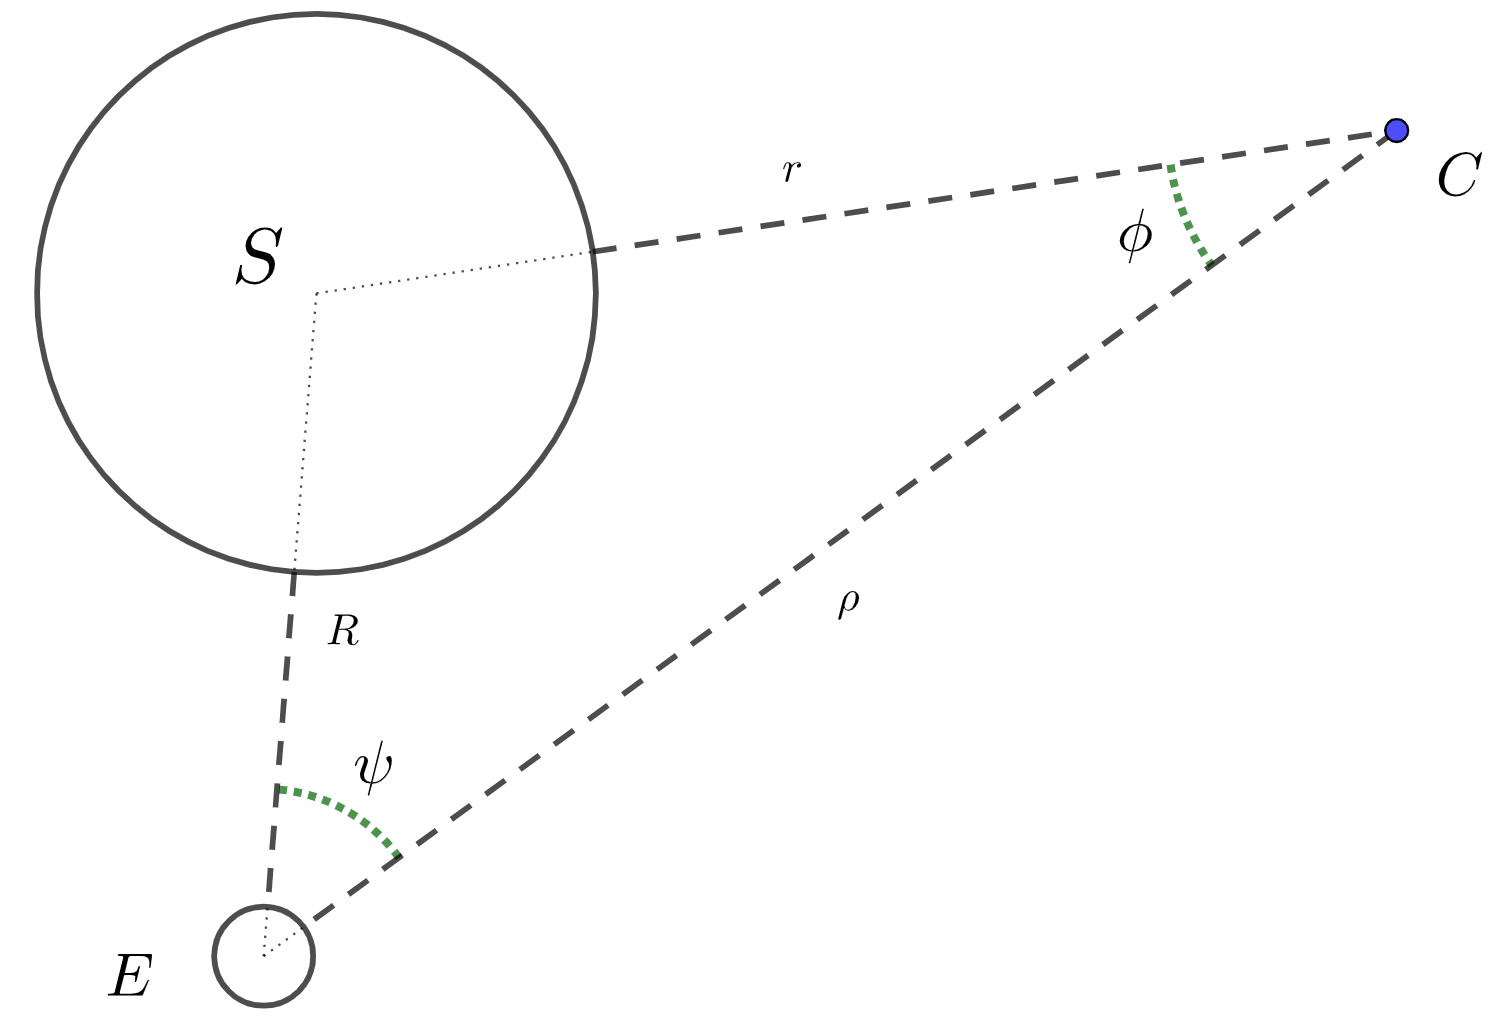
\includegraphics[scale=0.15]{images/notation_angles.png}
\caption{Triángulo formado por $S$, $E$ y $C$ junto a las distancias y ángulos generados.}
\label{fig:notation_angles}
\end{figure}

Nos encontramos ahora ante un problema de resolución de triángulos. A partir de la figura superior y del teorema de los senos ($\ddfrac{a}{\sin{\alpha}}=\ddfrac{b}{\sin{\beta}}=\ddfrac{c}{\sin{\gamma}}$), podemos escribir las siguientes ecuaciones:
\begin{align}
\left\{
\begin{array}{l}
	\rho=R\ddfrac{\sin{(\psi+\phi)}}{\sin{\phi}}\\
	r=R\ddfrac{\sin{\psi}}{\sin{\phi}}
\end{array}
\right.
\label{eq:triangle_relations_2}
\end{align}

Además, recordemos que podemos obtener el ángulo $\psi$ mediante:
\[
R\cos{\psi}=X\lambda+Y\mu+Z\nu\\
\]

\noindent obteniendo así que el valor de $\psi$ estará en el primer o cuarto cuadrante, pues $R>0$ y el producto escalar de $(X,Y,Z)$ por $(\lambda,\mu,\nu)$ es positivo. Pero, como nos encontramos en un triángulo, se ha de cumplir que $\psi<\pi$, y suponemos que el ángulo $\psi$ es agudo.\\

Si sustituimos las ecuaciones  \eqref{eq:triangle_relations_2} en la ecuación de $\rho$ en \eqref{eq:rho_values}, esta pasará a ser:
\[
R\sin{\psi}\cos{\phi}+\left(R\cos{\psi}-\ddfrac{D_1}{DR^3}\right)\sin{\phi}=\ddfrac{-D_1}{DR^3\sin^3{\psi}}\sin^4{\phi}
\]

\noindent de manera que, ya que podemos obtener el valor de $\psi$ utilizando la primera ecuación de \eqref{eq:triangle_relations_2}, nos queda una ecuación con una única incógnita, $\phi$.\\

Ahora, consideramos el vector en el plano $(R\cos{\psi}-\ddfrac{D_1}{DR^3},R\sin{\psi})$ y suponemos que es distinto del origen. Realmente esto ocurre siempre, ya que, como el ángulo $\psi$ es agudo y distinto de $0$, $R\sin{\psi}$ será distinto de $0$. Como consecuencia, al no ser el origen, podremos expresar dicho punto en coordenadas polares de la forma $N(\cos{m},\sin{m})$, con $N\neq0$ y pudiendo escoger el valor de $m$ en $(0,2\pi)$.\\

Con el fin de simplificar esta ecuación, definimos las siguientes expresiones:
\begin{align}
\left\{
\begin{array}{l}
	N\sin{m}=R\sin{\psi}\\
	N\cos{m}=R\cos{\psi}-\ddfrac{D_1}{DR^3}\\
	M=\ddfrac{-NDR^3\sin^3{\psi}}{D_1}
\end{array}
\right.
\label{eq:to_simplify}
\end{align}

Las dos primeras ecuaciones vienen dadas de la forma polar comentada anteriormente. Respecto a la tercera ecuación, la utilizaremos para darle un signo al valor $N$, de manera que podamos reducir el intervalo donde escoger el valor de $m$ a $(0,\pi)$. El signo de $N$ será elegido de tal manera que $M$ sea positivo, y como $\sin{\psi}>0$, $R>0$, el valor $N$ será positivo cuando $\ddfrac{D_1}{D}$ sea negativo y viceversa.\\

Hay ciertos casos excepcionales en las ecuaciones superiores. Si el término de la izquierda de la primera ecuación se anulase, llegaríamos a que $R\sin{\psi}=0$; como $R>0$ por definición, $\sin{\psi}=0$ y $\psi=k\pi$, $k\in\mathbb{Z}$, pero esta situación no es válida, pues entonces el sistema formado por el Sol, la Tierra y el objeto observado no formaría un triángulo tal y como queremos.\\

Fijado el signo de $M$, las dos primeras ecuaciones de \eqref{eq:to_simplify} determinarán unívocamente los valores $N$ y $m$, y la expresión que queríamos simplificar pasa a ser simplemente:
\begin{align}
\def\arraystretch{2}
\begin{array}{c}
	N\sin{m}\cos{\phi}+N\cos{m}\sin{\phi}=N\sin{(\phi+m)}=\ddfrac{N}{M}\sin^4{\phi} \Longrightarrow\\
	\Longrightarrow\sin^4{\phi}=M\sin{(\phi+m)}
\end{array}
\label{eq:phi_solution}
\end{align}

Aunque la ecuación \eqref{eq:phi_solution} podría estar definida para $\phi\in\mathbb{R}$, solo nos interesará en el intervalo $(0,\pi)$; es más, dicho intervalo se puede seguir reduciendo. Ya que $\phi$ es uno de los tres ángulos, y teniendo en cuenta cómo hemos definido $m$, podremos asegurar que $\phi=\pi-\psi$ es una solución válida (se puede comprobar sustituyendo en \eqref{eq:phi_solution}), aunque no es de valor práctico ya que que ésta corresponde a la posición del observador en la Tierra. Por tanto, dado que la solución ha de pertenecer al problema físico y que nos encontramos en un triángulo, podemos asegurar que:
\[
\phi<\pi-\psi
\]
\noindent y por tanto buscaremos una solución para la ecuación \eqref{eq:phi_solution}, no en todos los puntos que está definida, sino con $\phi$ estrictamente entre 0 y $\pi-\psi$.\\

Así, las soluciones de \eqref{eq:phi_solution} han de ser las intersecciones entre las curvas que definen las ecuaciones de la izquierda y de la derecha, es decir, la intersección entre:
\[
\left\{
\begin{array}{l}
	y_1=\sin^4{\phi}\\
	y_2=M\sin{(\phi+m)}
\end{array}
\right.
\]

Si el valor de $m$ es negativo cercano a cero y $M$ es ligeramente menor que 1, podemos ver la relación entre ambas curvas $y_1$, $y_2$ en la figura inferior:

\begin{figure}[H]
\centering
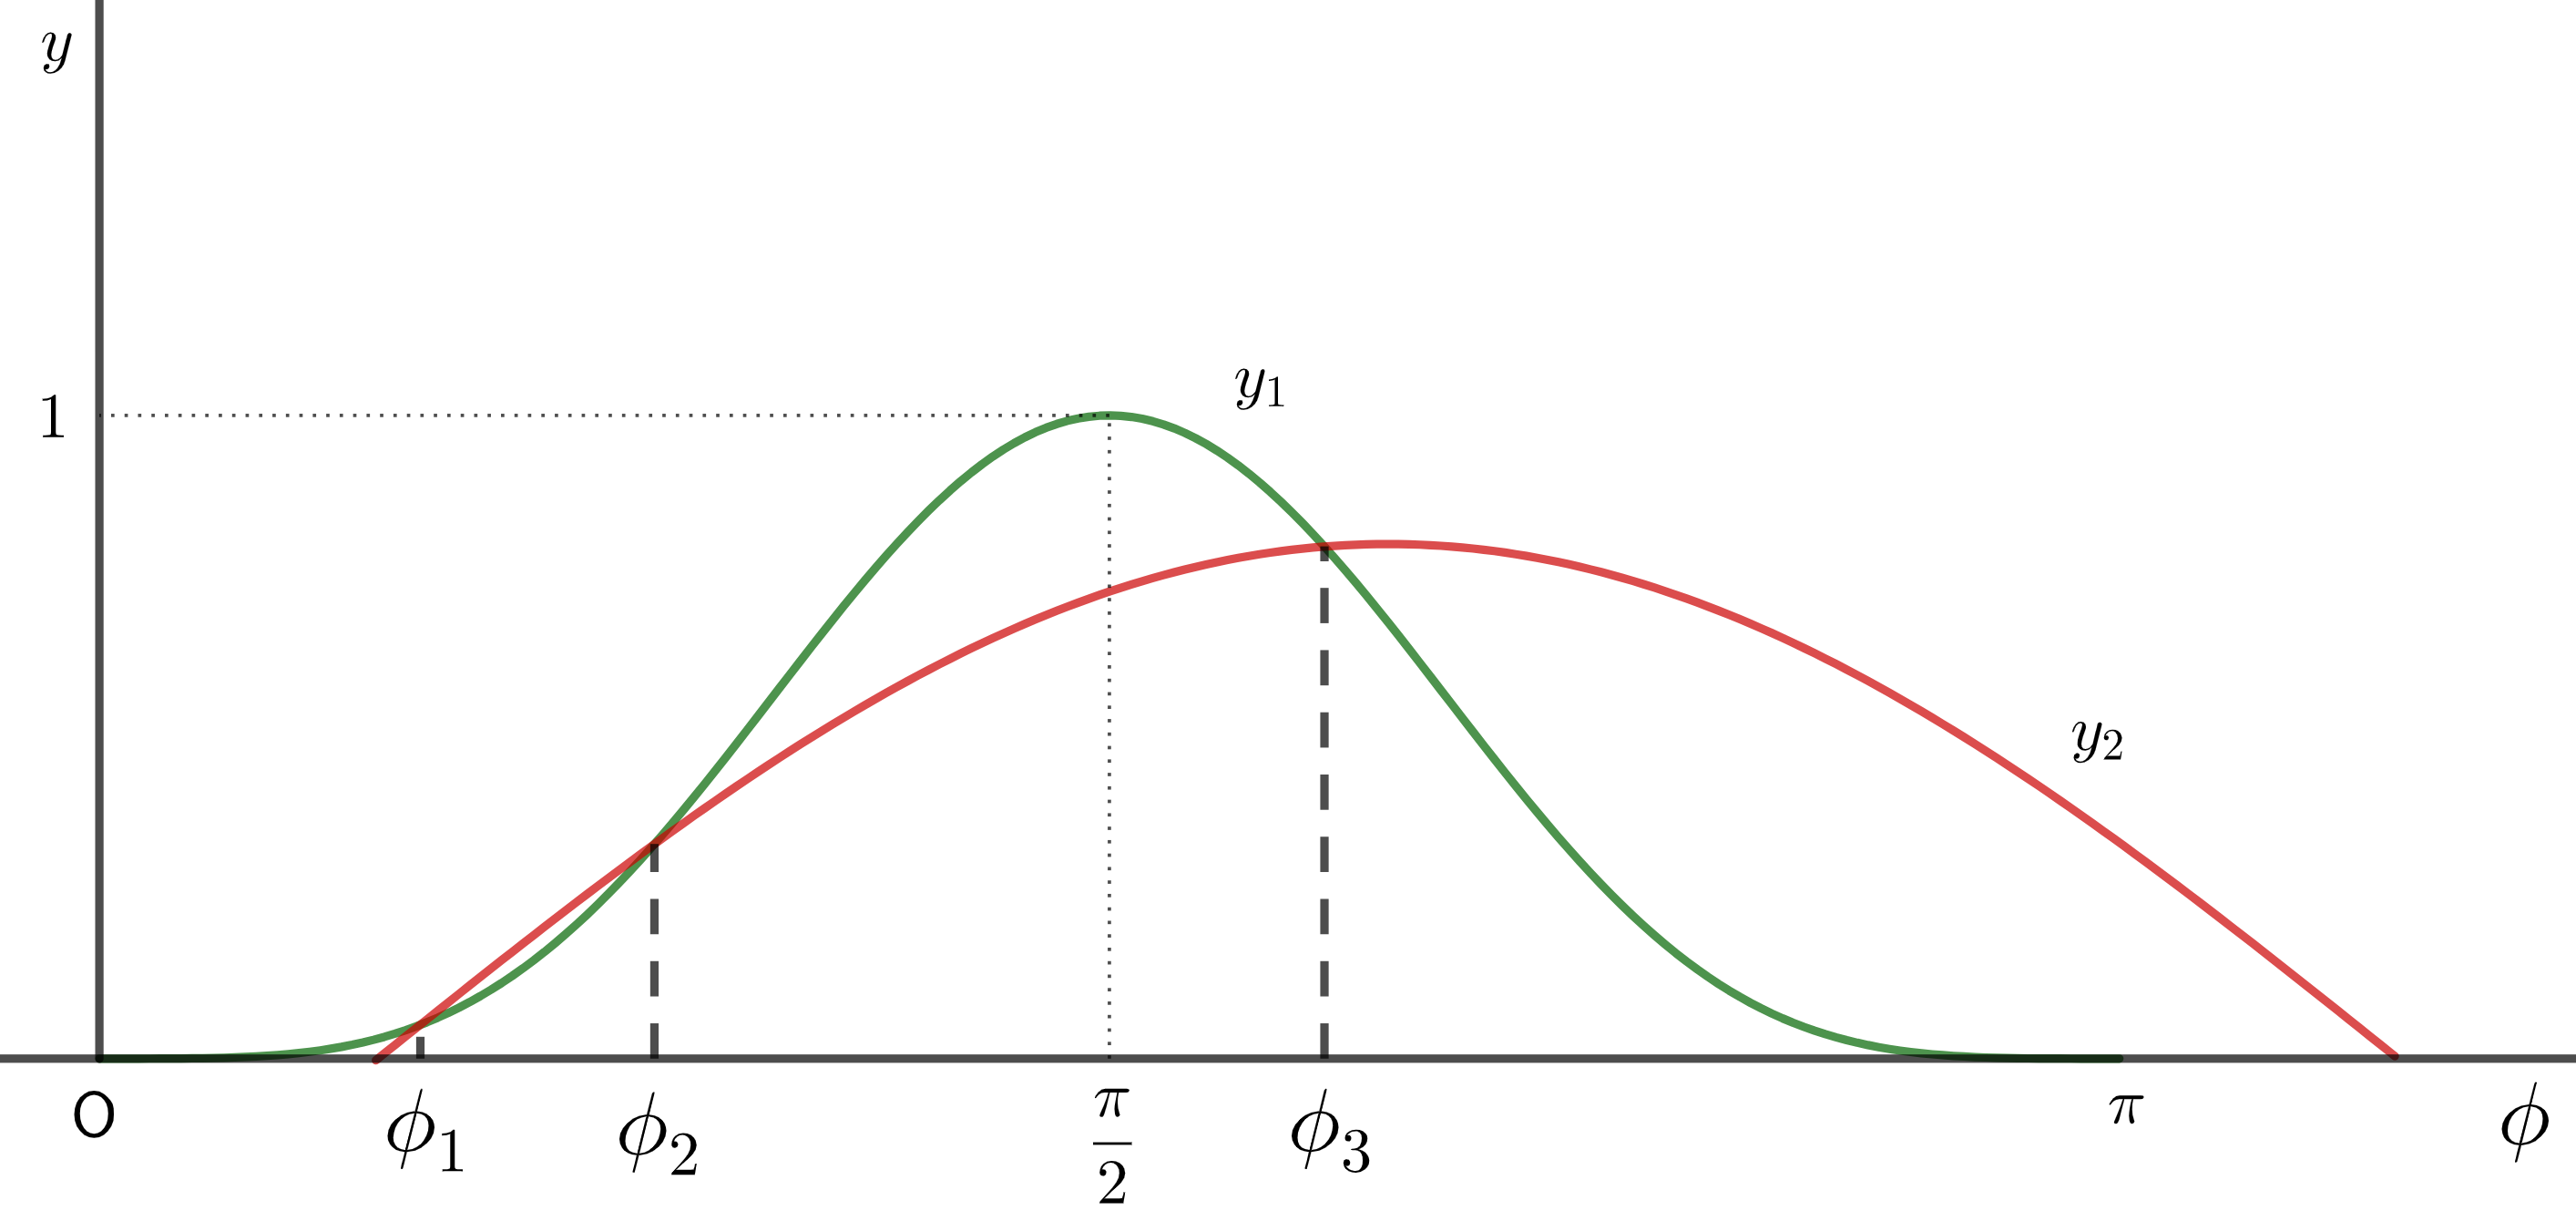
\includegraphics[scale=0.125]{images/phi_solution_m_negative_M_near_1.png}
\caption{Representación gráfica de $y_1$ e $y_2$ ($\frac{D_1}{D}>0$).}
\label{fig:phi_solution_m_negative_M_near_1}
\end{figure}

A partir de dicha imagen podemos observar que obtenemos tres intersecciones de las curvas, correspondientes cada una a una solución de \eqref{eq:phi_solution} y con $\phi_1<\phi_2<\phi_3$, sabiendo que una de ellas ha de ser $\pi-\psi$.\\

Discutamos ahora según el signo de $\frac{D_1}{D}$ los valores de $r$, $R$ y $m$. Comencemos considerando que $\frac{D_1}{D}$ es positivo. Es claro que $\rho$ y $r$ han de ser positivos, por lo que deducimos de la primera ecuación de \eqref{eq:rho_values} que $r$ ha de ser mayor que $R$. Por tanto, como $\psi$ ha de ser menor que 180º (pues estamos en un triángulo), utilizando las ecuaciones \eqref{eq:to_simplify} tenemos:
\[
\def\arraystretch{2}
\begin{array}{l}
M=\ddfrac{-NDR^3\sin^3{\psi}}{D_1}>0 \Longrightarrow N<0 \\
R\sin{\psi}>0 \Longrightarrow N\sin{m}>0 \Longrightarrow \sin{m}<0 \Longrightarrow m\in(\pi,2\pi)
\end{array}
\]

Por tanto, $N$ es negativo y $m$ estará en el tercer o cuarto cuadrante.\\

Si $m$ está en el cuarto cuadrante, la rama ascendente de la curva $y_2$ atraviesa el eje de abscisas $\phi$ en el primer cuadrante y, si $M<1$, las relaciones entre las dos curvas serán las que podemos ver en la figura \ref{fig:phi_solution_m_negative_M_near_1}. Si el valor de $m$ es cercano a 180º tendremos tres soluciones disponibles $\phi_1$, $\phi_2$, $\phi_3$, una de las cuales corresponderá al observador ($\phi_i=\pi-\psi$). Discutamos según cuál de las tres soluciones toma este valor:
\begin{itemize}
\item Si $\phi_1=\pi-\psi$, entonces el problema no tendría solución dado que cualquiera de las otras dos soluciones sería mayor que $\pi-\psi$.
\item Si $\phi_2=\pi-\psi$, se sigue del hecho de que $\phi<\pi-\psi$ que la solución ha de ser $\phi_1$ y es única.
\item Si $\phi_3=\pi-\psi$, las otras dos soluciones cumplirán todas las condiciones del problema, no pudiendo determinar cuál de las dos pertenece a la órbita real del cuerpo observado (siempre que no tengamos información adicional). Si tuviéramos una cuarta medición, repetiríamos el proceso anterior eliminando una de las mediciones tomadas y añadiendo ésta nueva; la solución que se repita (aproximadamente) será la perteneciente al problema real.

Pero, si solo dispusiésemos de tres mediciones, podría darse el caso de que los valores de $r$ y $\rho$ proporcionados por la solución $\phi_1$ fueran demasiado grandes como para que el objeto fuera visible para el observador, llegando así a la conclusión de que $\phi_2$, el cuál proporcionaría un $r$ más pequeño, pertenecería al problema físico.
\end{itemize} 

A medida que la rama ascendente de la curva $y_2$ se mueve hacia la derecha, es decir, fijando $M$ hacemos decrecer $m$, las soluciones $\phi_1$ y $\phi_2$ tienden a coincidir, y en estas condiciones el problema no tendría solución. Por tanto:
\begin{quote}
\textit{Si $\frac{D_1}{D}>0$, la distancia $r$ es mayor que $R$, el ángulo $m$ estará en el cuarto cuadrante y disponemos de una o dos soluciones del problema físico en función de que $\phi_2$ o $\phi_3$ sea igual a $\pi-\psi$.}\\
\end{quote}

Veamos ahora el caso contrario. 

\begin{figure}[H]
\centering
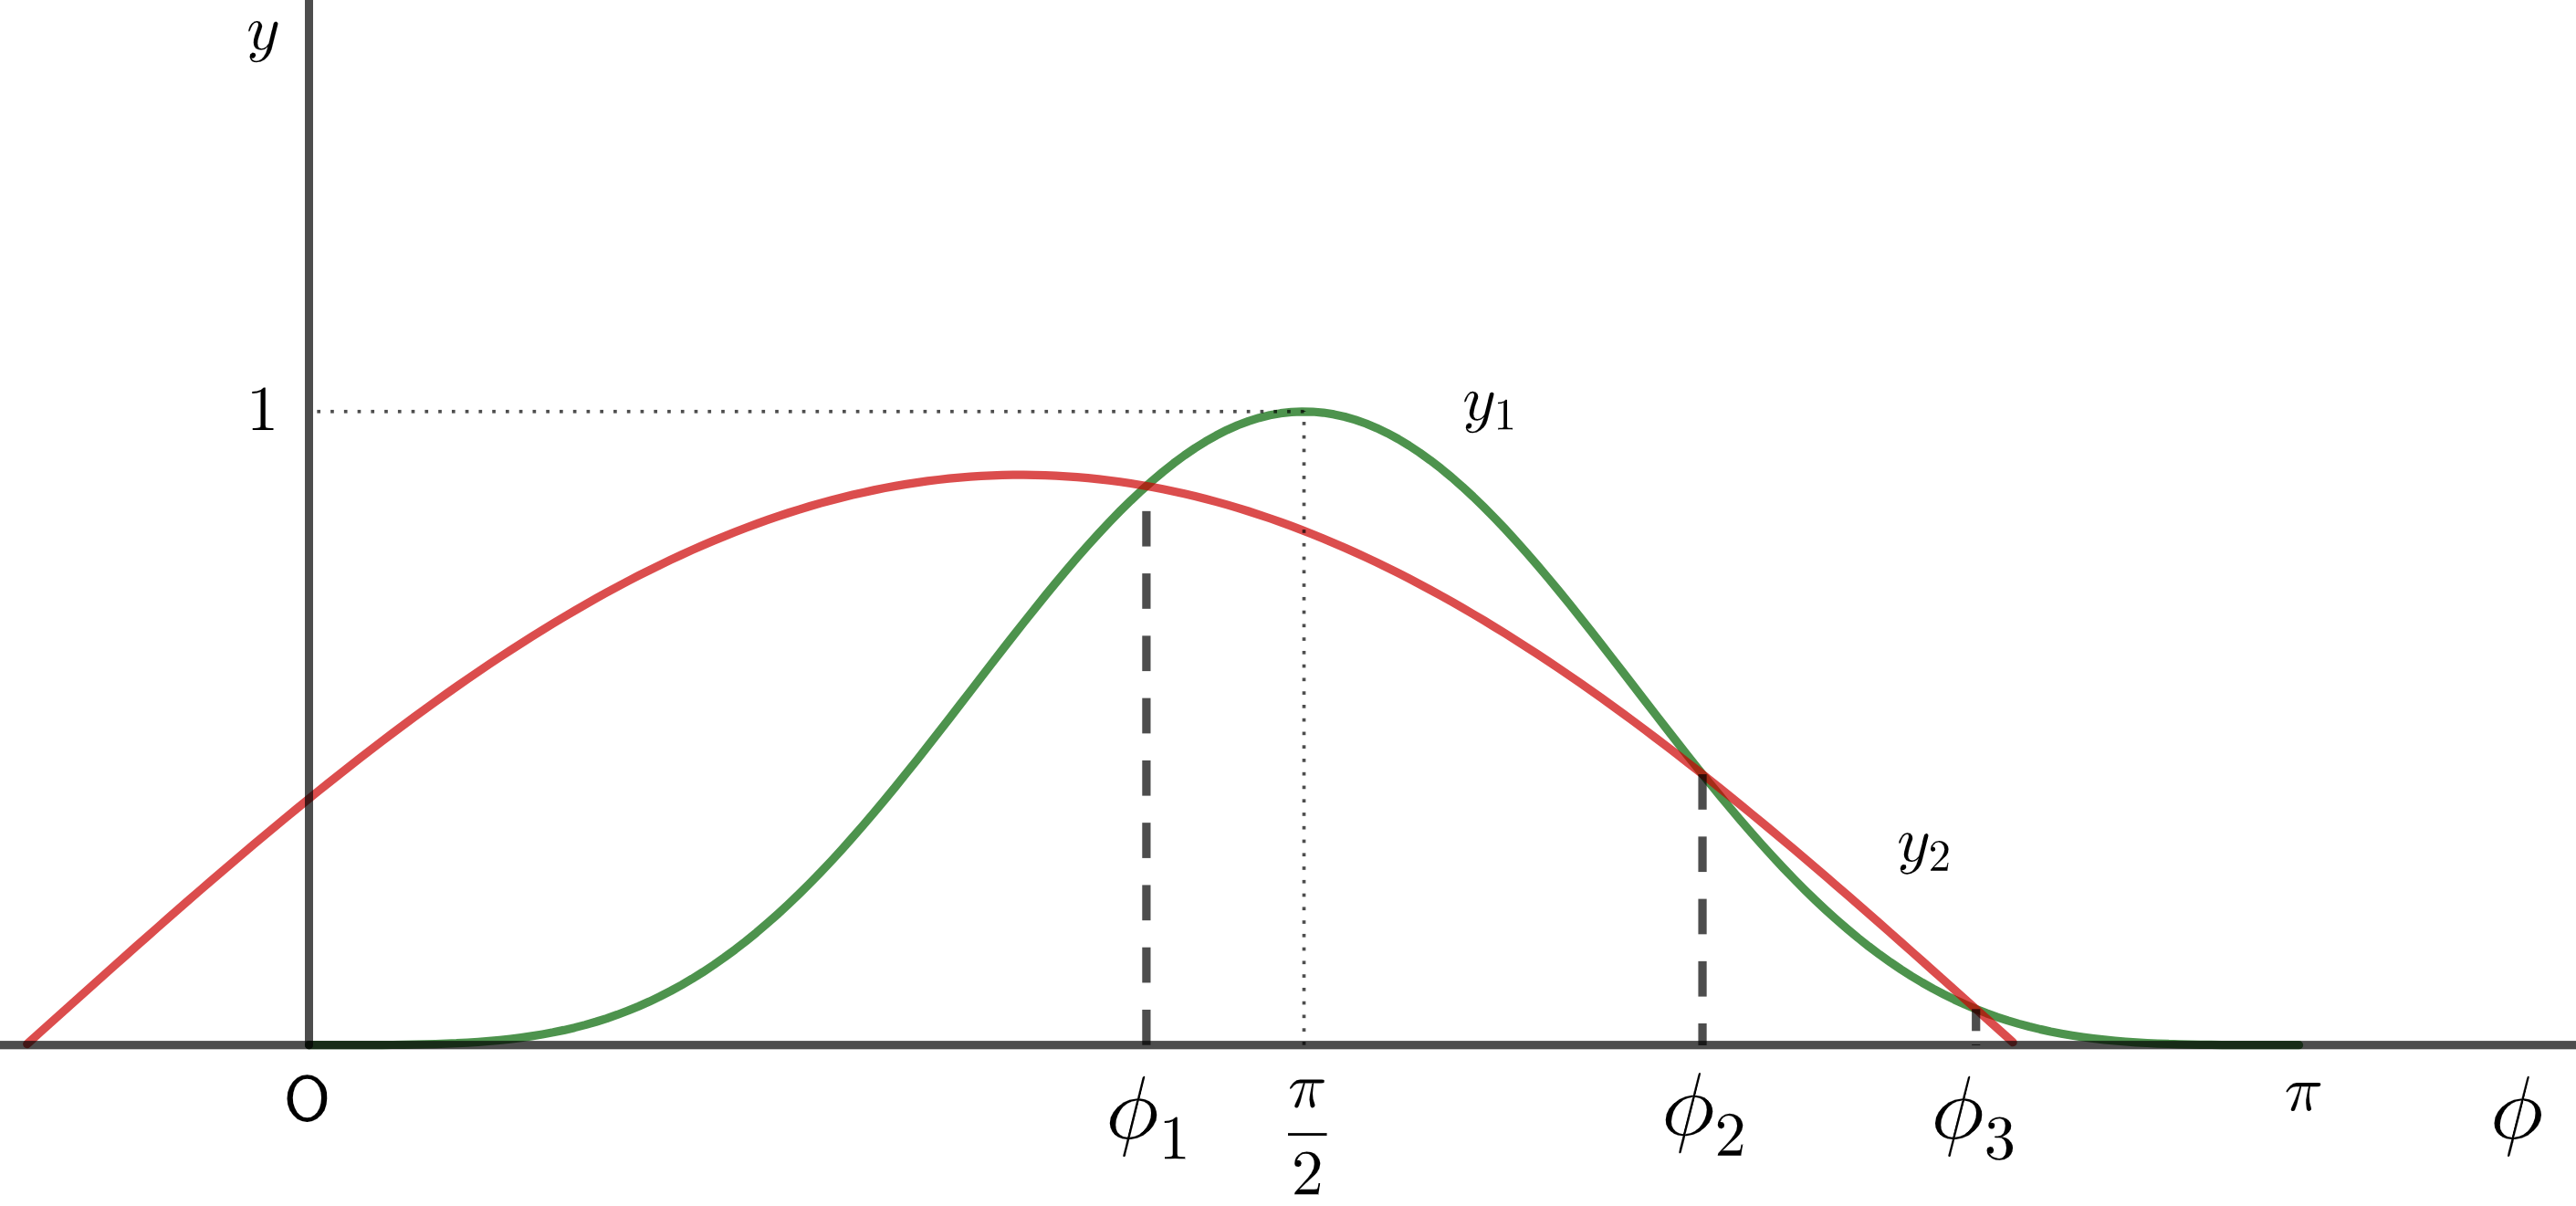
\includegraphics[scale=0.125]{images/phi_solution_m_positive_M_near_1.png}
\caption{Representación gráfica de $y_1$ e $y_2$ ($\frac{D_1}{D}<0$).}
\label{fig:phi_solution_m_positive_M_near_1}
\end{figure}

Supongamos que $\frac{D_1}{D}$ es negativo, de tal manera que, procediendo como en el caso positivo, llegamos a que $r<R$ y que $m$ está en el primer o segundo cuadrante. Si $m$ está en el primer cuadrante, la rama descendente de la curva $y_2$ atraviesa el eje de abscisas $\phi$ en el segundo cuadrante, y para un $m$ pequeño y $M<1$, las relaciones entre las dos curvas serán las que podemos ver en la gráfica \ref{fig:phi_solution_m_positive_M_near_1}. En este caso, la solución será única o doble en función de que $\phi_2$ o $\phi_3$ valgan $\pi-\psi$. Por último, si $m$ estuviera en el segundo cuadrante, la rama descendente de $y_2$ cortaría el eje de abscisas en el primer cuadrante, por lo que $\phi_2$ y $\phi_3$ no serían reales y el problema no tendría solución. Así, tenemos que:
\begin{quote}
\textit{Si $\frac{D_1}{D}<0$, la distancia $r$ es menor que $R$, el ángulo $m$ estará en el primer cuadrante y disponemos de una o dos soluciones del problema físico en función de que $\phi_2$ o $\phi_3$ sea igual a $\pi-\psi$.}\\
\end{quote}

Como consecuencia de toda esta discusión concluimos que, en determinadas situaciones, según las medidas que se nos den y el número de estas, nos encontraremos ante una única respuesta o dos respuestas, y en este segundo caso tendremos que discernir sobre cuál de las dos soluciones pertenecerá al problema físico.\\

%%%%%%%%%%%%%%%%%%%%%%%%%%%%%%%%

%%%%%%%%%%%%%%%%%%%%%%%%%%%%%%%%
\subsection{\normalfont{\textit{Aproximación numérica mediante el método de Newton.}}}
\label{subsec:newton_rhapson}
Tras haber realizado un estudio teórico de la ecuación \eqref{eq:phi_solution}, pasemos a buscar un método de resolución para ésta. Dado que no podemos encontrar valores exactos de $\phi$ que satisfagan la ecuación, pues no hay una fórmula explícita para la solución, utilizaremos el método de Newton para obtener un valor aproximado.\\

Considerando una función $f$ derivable y $x_0$ un valor inicial, definimos el método de Newton para cada $n$ como:
\[
x_{n+1}=x_n-\ddfrac{f(x_n)}{f'(x_n)}, n\geq0
\]

Para no aplicar la operación superior de forma infinita, impondremos una tolerancia $\delta$ a la hora de aplicar el método de manera que cuando $|x_{k+1}-x_k|<\delta$, la solución será $x_{k+1}$. Es necesario que $f'(x)\neq0$ para poder llevar este método a la práctica.\\

En nuestro caso, tomando $f(x)=\sin^4{x}-M\sin{(x+m)}$, tenemos que su derivada será $f'(x)=4\sin^3{x}\cos{x}-M\cos{(x+m)}$ de manera que la sucesión para la aproximación mediante el método de Newton será:
\begin{align}
x_{n+1}=x_n-\ddfrac{\sin^4{x_n}-M\sin{(x_n+m)}}{4\sin^3{x_n}\cos{x_n}-M\cos{(x_n+m)}}, \; \; \; \; \; n\geq0
\label{eq:phi_newton}
\end{align}

El método de Newton no siempre es convergente, por lo que es conveniente mencionar los teoremas de convergencia de este método. 
\begin{theorem}
\label{theo:convergence_newton}
Sea $f:I\rightarrow\mathbb{R}$ una función de clase 2 en un intervalo abierto $I$. Supongamos que existe $x^*$ tal que $f(x^*)=0$ y $f'(x^*)\neq0$; entonces, existe $\varepsilon>0$ tal que si $x_0\in[x^*-\varepsilon,x^*+\varepsilon]$, el método de Newton permite definir la sucesión $\{x_n\}_{n\in\mathbb{N}}$ que converge a $x^*$. Además, cuando $f''(x^*)\neq0$, dicha sucesión tiene orden de convergencia 2.\\
\end{theorem}

Dado que la función que queremos aproximar con el método de Newton es infinito-derivable por ser una función trigonométrica, podremos aplicar el teorema superior encontrado así el valor de $\phi$ para el que se cumple la ecuación \eqref{eq:phi_solution}.\\

Notemos que este teorema solo nos garantiza la convergencia supuesto que el punto $x_0$ sea cercano a la raíz, por lo que será buena idea separar las raíces por Bolzano y elegir el valor intermedio de los intervalos obtenidos como valor inicial para aplicar el método de Newton. La separación de raíces consiste en escoger un número adecuado de puntos $\alpha_1,...,\alpha_k\in[a,b]$ y aplicar el teorema de Bolzano para cada par $(\alpha_j,\alpha_{j+1})$, acotando así los intervalos donde buscar las raíces de una función. Ya que en nuestro caso buscamos la solución en el intervalo $[0,\pi]$ podremos escoger los puntos de la manera $\frac{j\cdot \pi}{n}$, con $j=0,...,n$, y una vez acotemos la raíz quedarnos como valor inicial:
\[
x_0=\ddfrac{\ddfrac{j\cdot\pi}{n}+\ddfrac{(j+1)\cdot\pi}{n}}{2}=\ddfrac{(2j+1)\cdot\pi}{2n}
\]

Veamos ahora un caso práctico de la aplicación de este método para determinar las soluciones de \eqref{eq:phi_solution}. Tomemos $M=0.6$ y $m=6$, por lo que $m$ estará en el cuarto cuadrante y nos encontraremos en el caso de \ref{fig:phi_solution_m_negative_M_near_1}. Escojamos $n=8$ y separemos las raíces en intervalos para escoger el valor de $x_0$.
\begin{table}[H]
\centering
\resizebox{9.5cm}{!}{%
\begin{tabular}{c|c|c|c|c|c|c|c|c|c}
$\alpha_j$    & $0$ & $\frac{\pi}{8}$ & $\frac{\pi}{4}$ & $\frac{3\pi}{8}$ & $\frac{\pi}{2}$ & $\frac{5\pi}{8}$ & $\frac{3\pi}{4}$ & $\frac{7\pi}{8}$ & $\pi$ \\ \hline
$f(\alpha_j)$ & + & -             & -             & +              & +             & +              & -              & -              & -  
\end{tabular}%
}
\end{table}

Tomamos, por ejemplo, el intervalo $[0,\frac{\pi}{8}]$ en el que nuestra función cambia de signo entre sus extremos. Calculamos el valor medio del intervalo, lo elegimos como valor inicial, $x_0=\frac{\pi}{16}$, y aplicamos el método de Newton con una tolerancia de $10^{-5}$. Veamos en una tabla cómo va convergiendo la solución.
\begin{table}[H]
\centering
\def\arraystretch{1.5}
\setlength{\tabcolsep}{20pt}
\begin{tabular}{ccc}
      &                       & $x_i-x_{i-1}$                   \\ \hline
$x_0$ & $\pi/16$              &                                 \\ \hline
$x_1$ & $0.2904116552751586$  & $0.0940621144257965$            \\ \hline
$x_2$ & $0.295092645742656$   & $0.00468099046749737$           \\ \hline
$x_3$ & $0.29511191583666796$ & $1.92700940119805\cdot10^{-5}$  \\ \hline
$x_4$ & $0.29511191616986304$ & $3.33195082635740\cdot10^{-10}$ \\ \hline
\end{tabular}
\end{table}

Por tanto, en cuatro iteraciones del método la diferencia entre las soluciones obtenidas es menor a la tolerancia que hemos fijado, obteniendo así que $\phi_1=0.29511191616986304$ es una solución de \eqref{eq:phi_solution}. De la misma manera calcularemos las raíces $\phi_2$ en $[\frac{\pi}{4},\frac{3\pi}{8}]$ y $\phi_3$ en $[\frac{5\pi}{8},\frac{3\pi}{4}]$.\\

Tras aplicar el método de Newton y haber obtenido todas las soluciones de \eqref{eq:phi_solution} en el intervalo $[0,\pi]$, nos faltará comprobar cuál de las soluciones obtenidas es igual a $\pi-\psi$, pudiendo determinar así si hay o no unicidad para el problema físico. Aún así, es posible determinar la unicidad de la solución sin necesidad de resolver la ecuación \eqref{eq:phi_solution}, como veremos a continuación.\\

\subsection{\normalfont{\textit{Unicidad de la solución.}}}
\label{subsec:unicidad}
Tal y como hemos visto en la sección anterior, la solución del problema físico será única si $\phi_2=\pi-\psi$, independientemente del signo de $\frac{D_1}{D}$; en otro caso, la solución será doble o no existirá.\\

Fijémonos en la figura \ref{fig:phi_solution_m_negative_M_near_1}, donde aparecen tres intersecciones entre las curvas $y_1$ e $y_2$. La observación fundamental en esta gráfica reside en el hecho de que $\phi_2$ es un cero positivo, entendiendo por esto que la derivada en dicho punto es positiva, es decir, la función es creciente, y $\phi_1$ y $\phi_3$ son ceros negativos. Podemos ver esto más fácilmente en la siguiente imagen:

\begin{figure}[H]
\centering
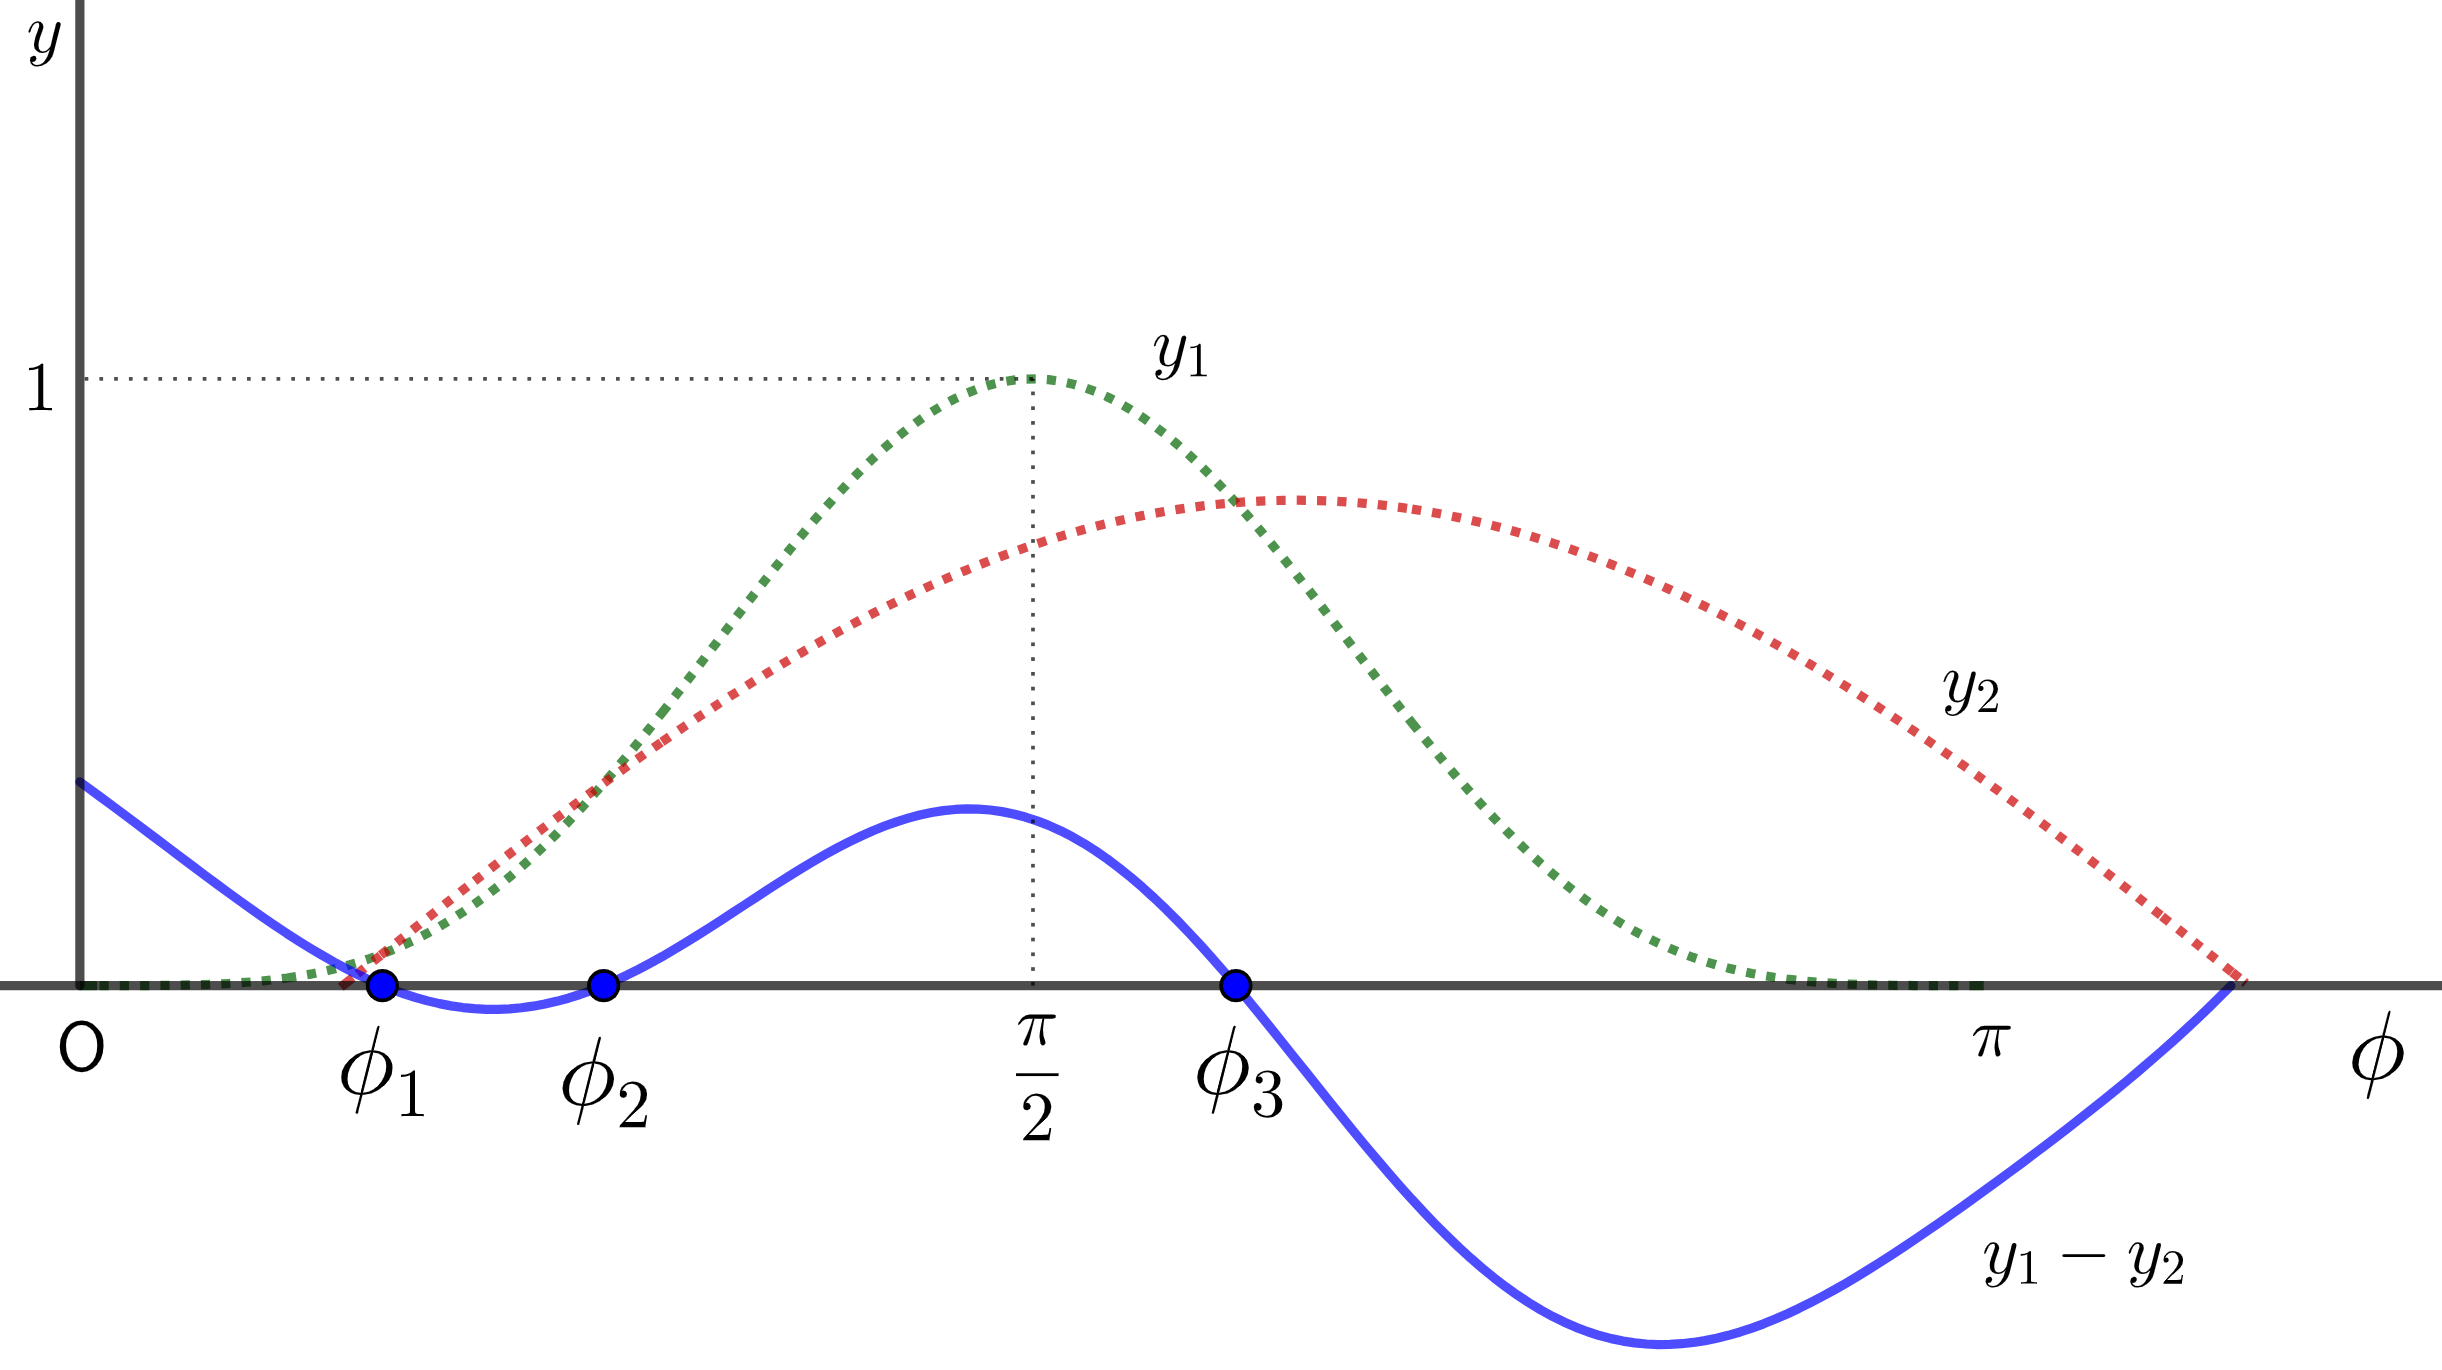
\includegraphics[scale=0.125]{images/y_1_menos_y_2.png}
\caption{Representación gráfica de $y_1-y_2$ cuando $\ddfrac{D_1}{D}>0$.}
\label{fig:y_1_menos_y_2}
\end{figure}

Por otra parte, calculemos la derivada de $y_1-y_2$:
\[
(y_1-y_2)'(x)=4\sin^3{\phi}\cos{\phi}-M\cos{(\phi+m)}
\]

Pues bien, para que nuestra solución sea única tendrá que cumplirse que la derivada de $y_1-y_2$ en el punto $\pi-\psi$ sea positiva, es decir, que $\phi_2=\pi-\psi$. Desarrollemos la derivada en este punto para comprobar más fácilmente en qué casos se cumple la unicidad.
\[
\def\arraystretch{2}
\begin{array}{ll}
  & 4\sin^3{(\pi-\psi)}\cos{(\pi-\psi)}-M\cos{(\pi-\psi+m)}=\\
= &-4\sin^3{(\pi-\psi)}\cos{\psi}+M\cos{(-\psi+m)}=\\
= & \left[\ddfrac{4MD_1}{NDR^3}\cos{\psi}+M(\cos{\psi}\cos{m}+\sin{\psi}\sin{m})\right]=\\
= & \ddfrac{4MD_1}{NDR^3}\cos{\psi}+M\left(\ddfrac{R\cos^2{\psi}}{N}-\ddfrac{D_1\cos{\psi}}{NDR^3}+\ddfrac{R\sin^2{\psi}}{N}\right)=\\
= & \ddfrac{4MD_1}{NDR^3}\cos{\psi}-\ddfrac{MD_1}{NDR^3}\cos{\psi}+\ddfrac{MR}{N}(\cos^2{\psi}+\sin^2{\psi})=\\
= & \ddfrac{MR}{N}\left(1+\ddfrac{3D_1}{DR^4}\cos{\psi}\right)
\end{array}
\]

Dado que $M$ y $R$ son valores positivos podremos obviarlos a la hora de escribir la desigualdad. Así, tenemos una condición de unicidad para el caso de la figura \ref{fig:phi_solution_m_negative_M_near_1}, es decir, cuando $\ddfrac{D_1}{D}$ sea positivo, facilitando así un estudio previo en la determinación del ángulo $\phi$.\\

El razonamiento para $\ddfrac{D_1}{D}<0$ es análogo; en este caso, $\phi_2$ será un cero negativo y las otras dos soluciones serán ceros positivos, por lo que tendremos que comprobar que la derivada en $\pi-\psi$ sea negativa.\\

Así, con las dos desigualdades que hemos obtenido, llegamos a la conclusión de que la condición para que el problema físico tenga solución única es:
\begin{align}
\left\{
\def\arraystretch{2}
\begin{array}{l}
	\ddfrac{1}{N}\left[1+\ddfrac{3D_1}{DR^4}\cos{\psi}\right]>0 \; \; \; \; \text{si} \; \; \; \; \ddfrac{D_1}{D}>0\\
	\ddfrac{1}{N}\left[1+\ddfrac{3D_1}{DR^4}\cos{\psi}\right]<0 \; \; \; \; \text{si} \; \; \; \; \ddfrac{D_1}{D}<0
\end{array}
\right.
\label{eq:condicion_unicidad}
\end{align}

Dado que todos los valores de estas ecuaciones están dados por simples observaciones, no será necesario resolver la ecuación \eqref{eq:phi_solution} para determinar la unicidad de la solución.\\

Sabemos que $N\neq0$, y por tanto el límite de las dos desigualdades será:
\[
\left[1+\ddfrac{3D_1}{DR^4}\cos{\psi}\right]=0
\]

Ahora, utilicemos \eqref{eq:rho_values} y la relación \eqref{eq:triangle_relations_1} para eliminar $\cos{\psi}$ y $\frac{D_1}{D}$ de la expresión superior.
\[
\left\{
\def\arraystretch{2}
\begin{array}{l}
	\cos{\psi}=\ddfrac{r^2-\rho^2-R^2}{-2\rho R}\\
	\ddfrac{D_1}{D}=\ddfrac{\rho}{\left(\ddfrac{1}{R^3}-\ddfrac{1}{r^3}\right)}
\end{array}
\right.
\]
\[
\def\arraystretch{2}
\begin{array}{ll}
& 1+\ddfrac{3}{R^4}\ddfrac{\rho}{\left(\ddfrac{1}{R^3}-\ddfrac{1}{r^3}\right)}\ddfrac{r^2-\rho^2-R^2}{-2\rho R}=0\\
\Longrightarrow & \ddfrac{3\rho}{\left(\ddfrac{1}{R^3}-\ddfrac{1}{r^3}\right)}(r^2-\rho^2-R^2)=2\rho R^5\\
\Longrightarrow & r^2-\rho^2-R^2=\ddfrac{2}{3}R^5\left(\ddfrac{1}{R^3}-\ddfrac{1}{r^3}\right)
\end{array}
\]

Obtenemos así la igualdad:
\begin{align}
\rho^2=r^2+\ddfrac{2}{3}\ddfrac{R^5}{r^3}-\ddfrac{5}{3}R^2
\label{eq:rho_cuadrado}
\end{align}

Tomemos el miembro de la derecha de esta igualdad como una ecuación en $r$ y calculemos sus extremos mediante el método clásico:
\[
\ddfrac{\partial}{\partial r} (r^2+\ddfrac{2}{3}\ddfrac{R^5}{r^3}-\ddfrac{5}{3}R^2)=2r-\ddfrac{2R^5}{r}=0 \Longrightarrow R=r
\]

Por tanto, tenemos un extremo en $r=R$, que comprobaremos si es máximo o mínimo derivando una vez más:
\[
\ddfrac{\partial^2}{\partial r^2}(r^2+\ddfrac{2}{3}\ddfrac{R^5}{r^3}-\ddfrac{5}{3}R^2)=\ddfrac{8R^5}{r^5}+2
 \; \; \; \xRightarrow[]{r=R} \; \; \; \ddfrac{8R^5}{R^5}+2>0, \; \; \; \forall R>0
\]

Así, tenemos un mínimo para nuestra función en $r=R$, y dado que el mínimo valor que puede tomar $R$ es cero, el miembro de la derecha de \eqref{eq:rho_cuadrado} alcanzará el mínimo en $r=0$, por lo que para cada valor de $r$ habrá un único valor positivo de $\rho$. Además, dado que estamos trabajando con el límite de las desigualdades \eqref{eq:condicion_unicidad}, todos los pares de valores $(\rho,r)$ que satisfagan la igualdad \eqref{eq:rho_cuadrado} se encontrarán en el límite de las regiones donde la solución es única, las cuales son superficies de revolución alrededor de la línea imaginaria que une la Tierra y el Sol. Intentemos entender esto mejor mediante una imagen.
\begin{figure}[H]
\centering
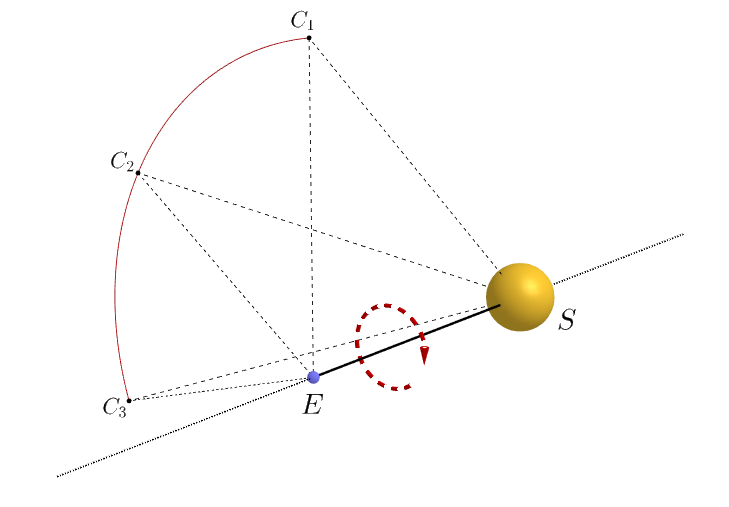
\includegraphics[scale=0.4]{images/eje_rotacion.png}
\caption{Distintas posiciones del cuerpo $C$, todas con las mismas distancias, $r$ y $\rho$, desde éstas al Sol y la Tierra.}
\label{fig:eje_rotacion}
\end{figure}

Dado que $r$ y $\rho$ son distancias del Sol y la Tierra al cuerpo observado, habrá infinitos puntos en el espacio tridimensional donde estos valores se mantengan. En la imagen superior podemos ver como, girando en torno a un círculo cuyo eje es el vector $\vec{SE}$, la distancia de cada $C_i$ es la misma independientemente de en qué punto del círculo se encuentre. Por tanto, volviendo a lo comentado anteriormente, podremos formar una superficie de revolución para el límite de las regiones donde la solución pasa a ser única tomando los pares $(\rho,r)$ en dicho límite y girando alrededor de vector $\vec{SE}$.

\begin{figure}[H]
\centering
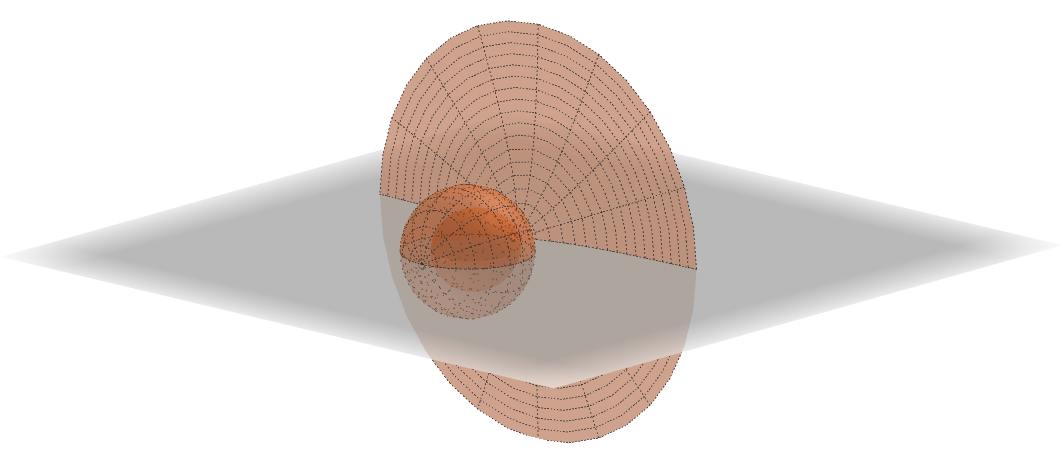
\includegraphics[scale=0.35]{images/sup_revol.png}
\caption{Superficie formada por los límites donde cambia la unicidad de la solución.}
\label{fig:sup_revol}
\end{figure}

En la imagen superior el círculo grande se extenderá hasta el infinito. A continuación, para obtener una imagen más visual en la que estudiar el cambio en la unicidad de la solución al atravesar las regiones límite, representamos una sección de la superficie con un plano que pase por la recta $SE$.
\begin{figure}[H]
\centering
\subfloat{
	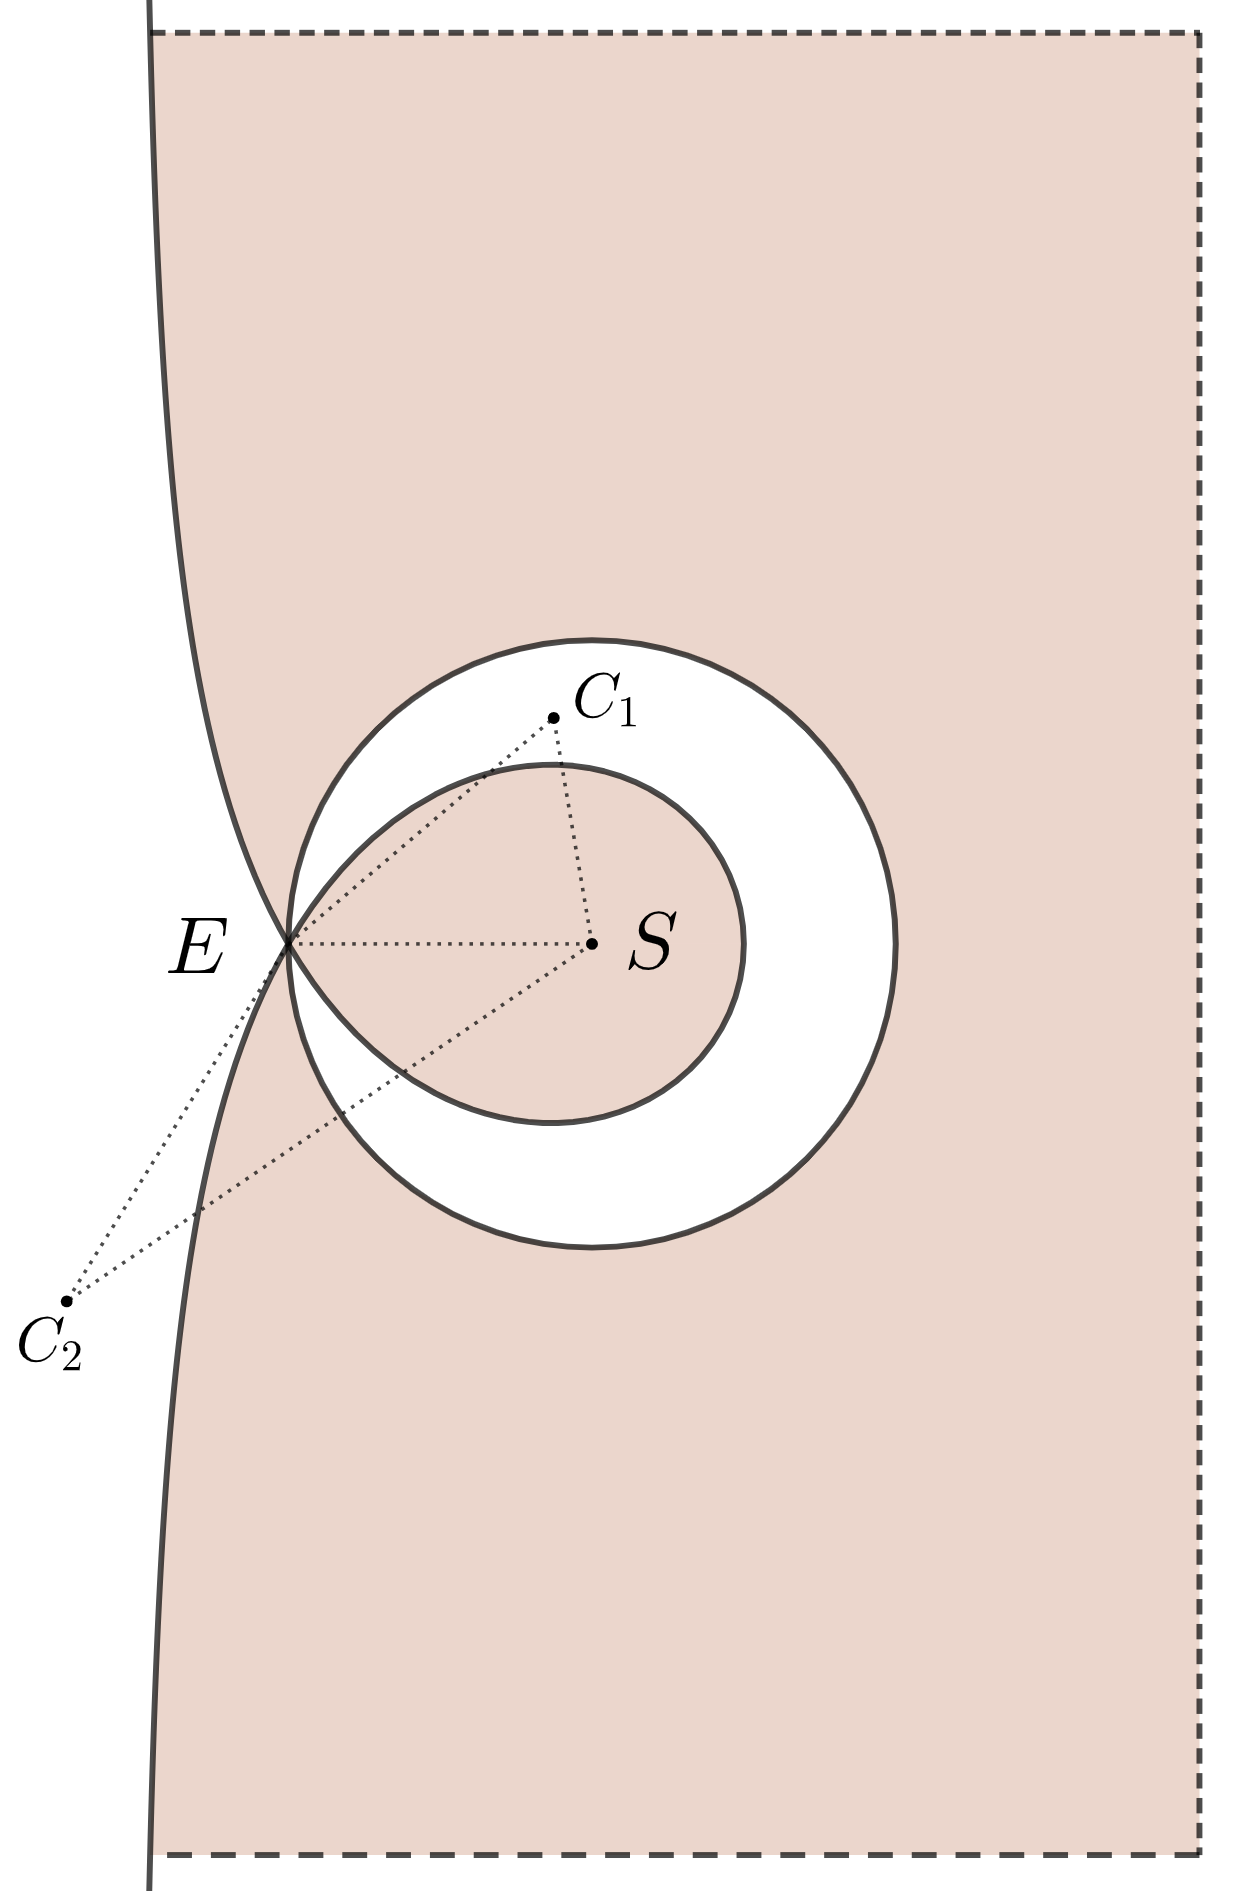
\includegraphics[scale=0.1]{images/seccion_superficie_unicidad.png}
	\hspace{1cm}
	\rulesep
	\hspace{1cm}
	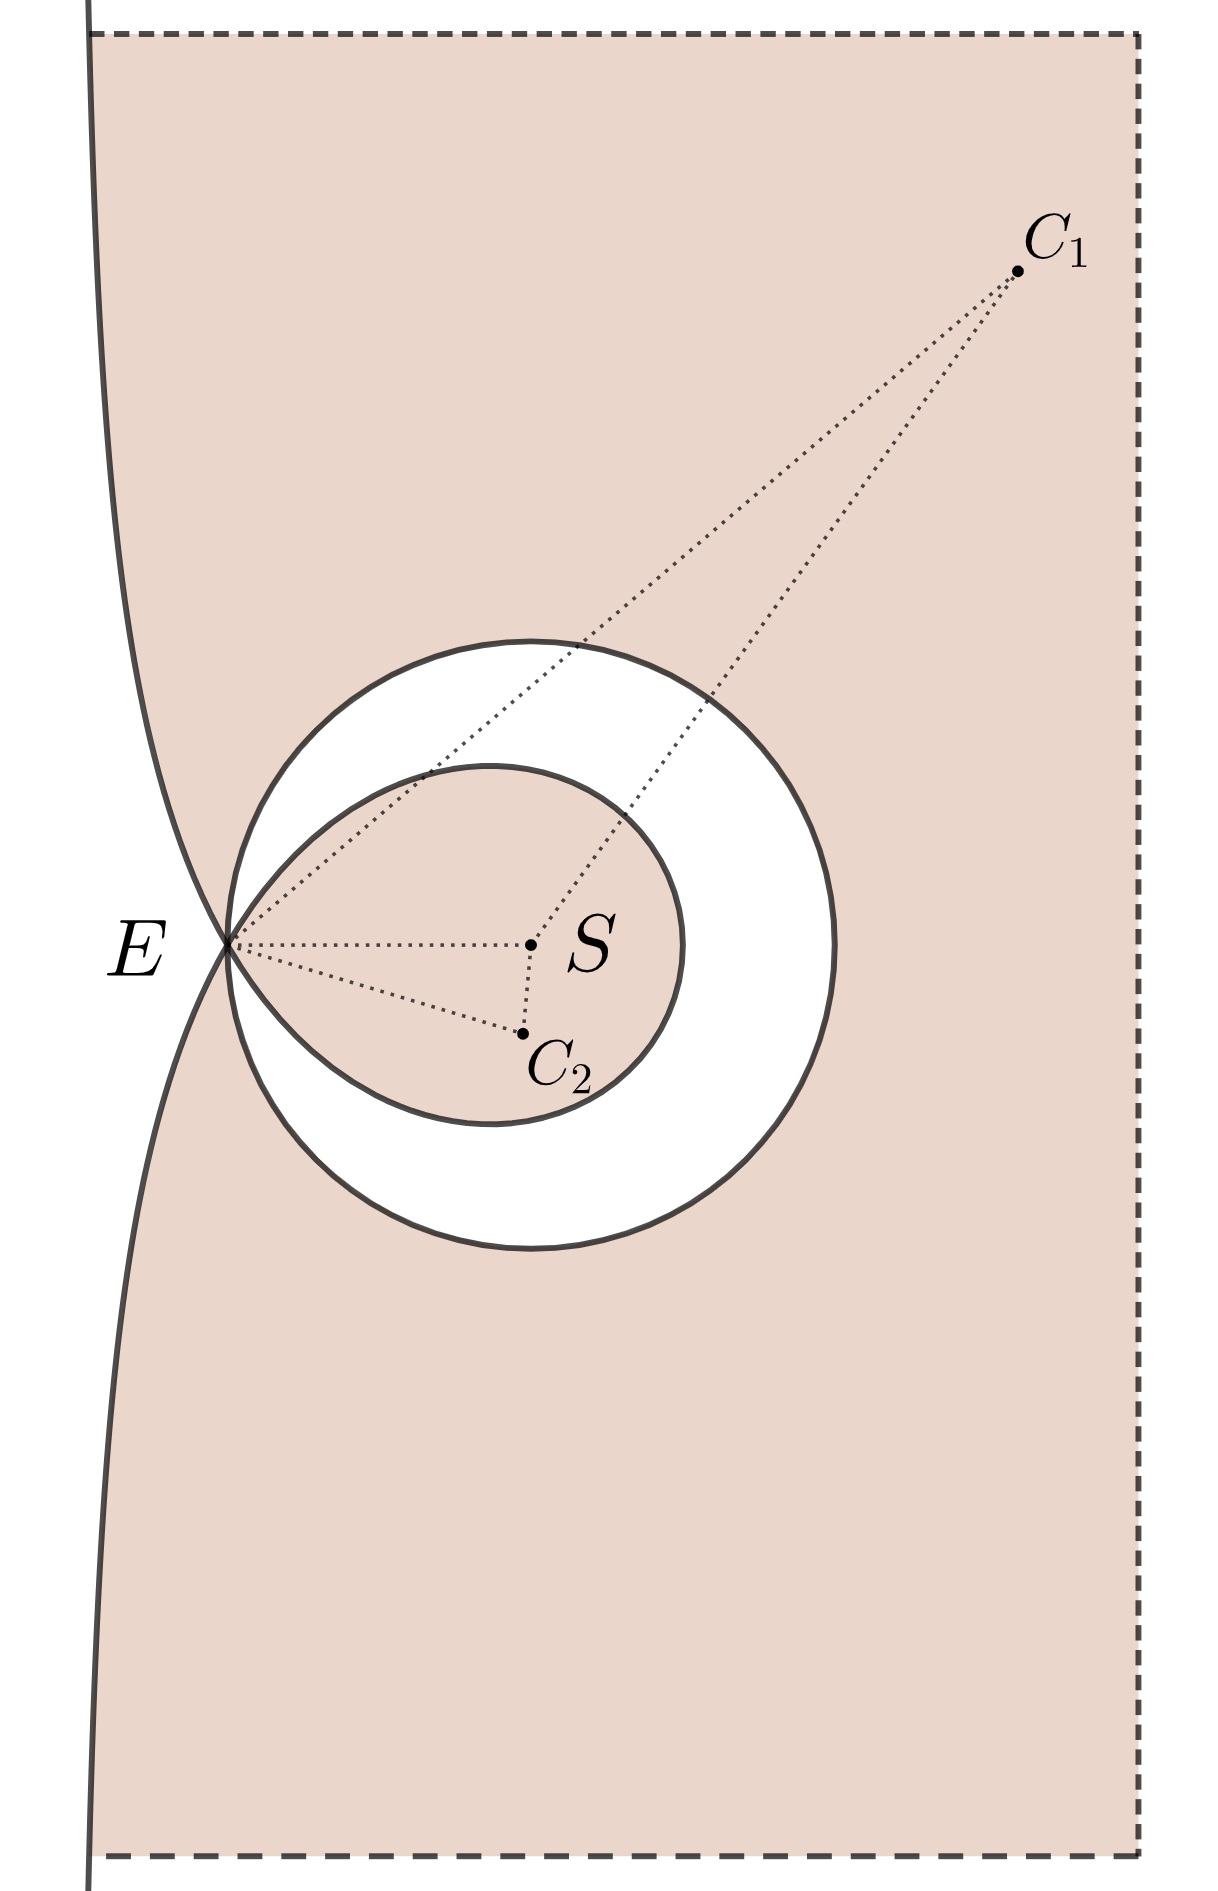
\includegraphics[scale=0.1]{images/seccion_superficie_no_unicidad.png}
}
\caption{Sección de la superficie de revolución junto a los casos en los que se da la unicidad y los que no. La región rosa se sigue extendiendo hasta el infinito.}
\label{fig:seccion_superficie}
\end{figure}

En la imagen superior podemos ver que los límites para la condición de unicidad dividen el espacio en cuatro partes diferentes, dos sombreadas y las otras dos en blanco, de manera que las desigualdades de \eqref{eq:condicion_unicidad} mantienen el signo dentro de cada una de estas regiones y cambian de signo al cruzar la frontera de alguna de ellas.\\

Estudiemos ahora en cuál de estas regiones obtenemos una solución única y en cual doble. Para ello, tomemos un punto a la izquierda de $E$ en la recta $SE$, en el cuál se cumplirá que $r=\rho+R$ y $\psi=\pi$. Con esto, comprobemos la unicidad con \eqref{eq:condicion_unicidad}:
\[
\def\arraystretch{2}
\begin{array}{ll}
  & 1+\ddfrac{3D_1}{DR^4}\cos{\psi} = 1-\ddfrac{3D_1}{DR^4} = 1-\ddfrac{3}{R^4}\ddfrac{\rho}{\left(\ddfrac{1}{R^3}-\ddfrac{1}{r^3}\right)} = \\
= & 1-\ddfrac{3\rho}{R-\ddfrac{R^4}{r^3}} = 1-\ddfrac{3\rho}{R-\ddfrac{R^4}{(\rho+R)^3}} = 1-\ddfrac{3\rho}{\ddfrac{R(\rho+R)^3-R^4}{(\rho+R)^3}} = \\
= & 1-\ddfrac{3\rho(\rho+R)^3}{\rho^3R+3\rho^2R^2+3\rho R^3+R^4-R^4} = 1-\ddfrac{3(\rho+R)^3}{R(\rho^2+3\rho R+3R^2)}
\end{array}
\]

Podemos ver fácilmente que esta última igualdad es negativa para un valor grande de $\rho$, y ya que hemos supuesto previamente que $r>R$, se sigue que $\ddfrac{D_1}{D}>0$ y $N<0$, por lo que estamos en la primera desigualdad de \eqref{eq:condicion_unicidad}. Ya que esta desigualdad está satisfecha, podemos concluir que la solución del problema será única si el objeto observado se encuentra en el área no sombreada a la izquierda de $E$.\\

Cuando el objeto cruce de la región no sombreada a la izquierda de \ref{fig:seccion_superficie} a una región sombreada, manteniendo que $r>R$, la función cambiará de signo mientras que el signo de $N$ no cambie, en cuyo caso la primera desigualdad de \eqref{eq:condicion_unicidad} no se cumplirá y estaremos en el caso de una solución doble. En esta región, la primera función de \eqref{eq:condicion_unicidad} es positiva y $N$ es negativo, por lo que si cruzamos al área pequeña sin sombra la función pasa a ser negativa y $N$ positivo, satisfaciendo así la segunda desigualdad y deduciendo así que la solución es única. De manera similar, podremos comprobar que la solución es doble en la región sombreada pequeña.\\

Por tanto, el problema físico tiene solución única en los casos que vemos en la primera imagen de \ref{fig:seccion_superficie}, es decir, en las regiones blancas, y solución doble en los casos de la segunda imagen, las regiones sombreadas.\\



\subsection{\normalfont{\textit{Límites en $m$ y $M$.}}}
\label{subsec:limites_m_M}
A la hora de determinar una órbita en un problema real, hemos de tener en cuenta que los valores $m$ y $M$ han de cumplir que las soluciones reales de la ecuación \eqref{eq:phi_solution} estén entre $0$ y $\pi$, pues sino el Sol, la Tierra y el objeto observado no formarían un triángulo. Por tanto, hemos de determinar los límites para que esta condición se satisfaga, y dichos límites pueden ser determinados mediante las condiciones para que obtengamos raíces dobles.\\

Para empezar, supongamos que $M$ es un valor fijo mientras $m$ varía. En el primer caso, que podemos ver en \ref{fig:phi_solution_m_negative_M_near_1}, se observan tres intersecciones de las curvas. Mientras $m$ vaya disminuyendo, la curva $y_2$ irá desplazándose hacia la derecha hasta que $\phi_1$ y $\phi_2$ pasen a ser iguales, teniendo así una raíz doble. De la misma manera, en \ref{fig:phi_solution_m_positive_M_near_1} observamos tres soluciones y, conforme $m$ aumente y desplace $y_2$ a la izquierda, $\phi_2$ y $\phi_3$ se igualarán.\\

\begin{figure}[H]
\centering
%\subfloat{
%	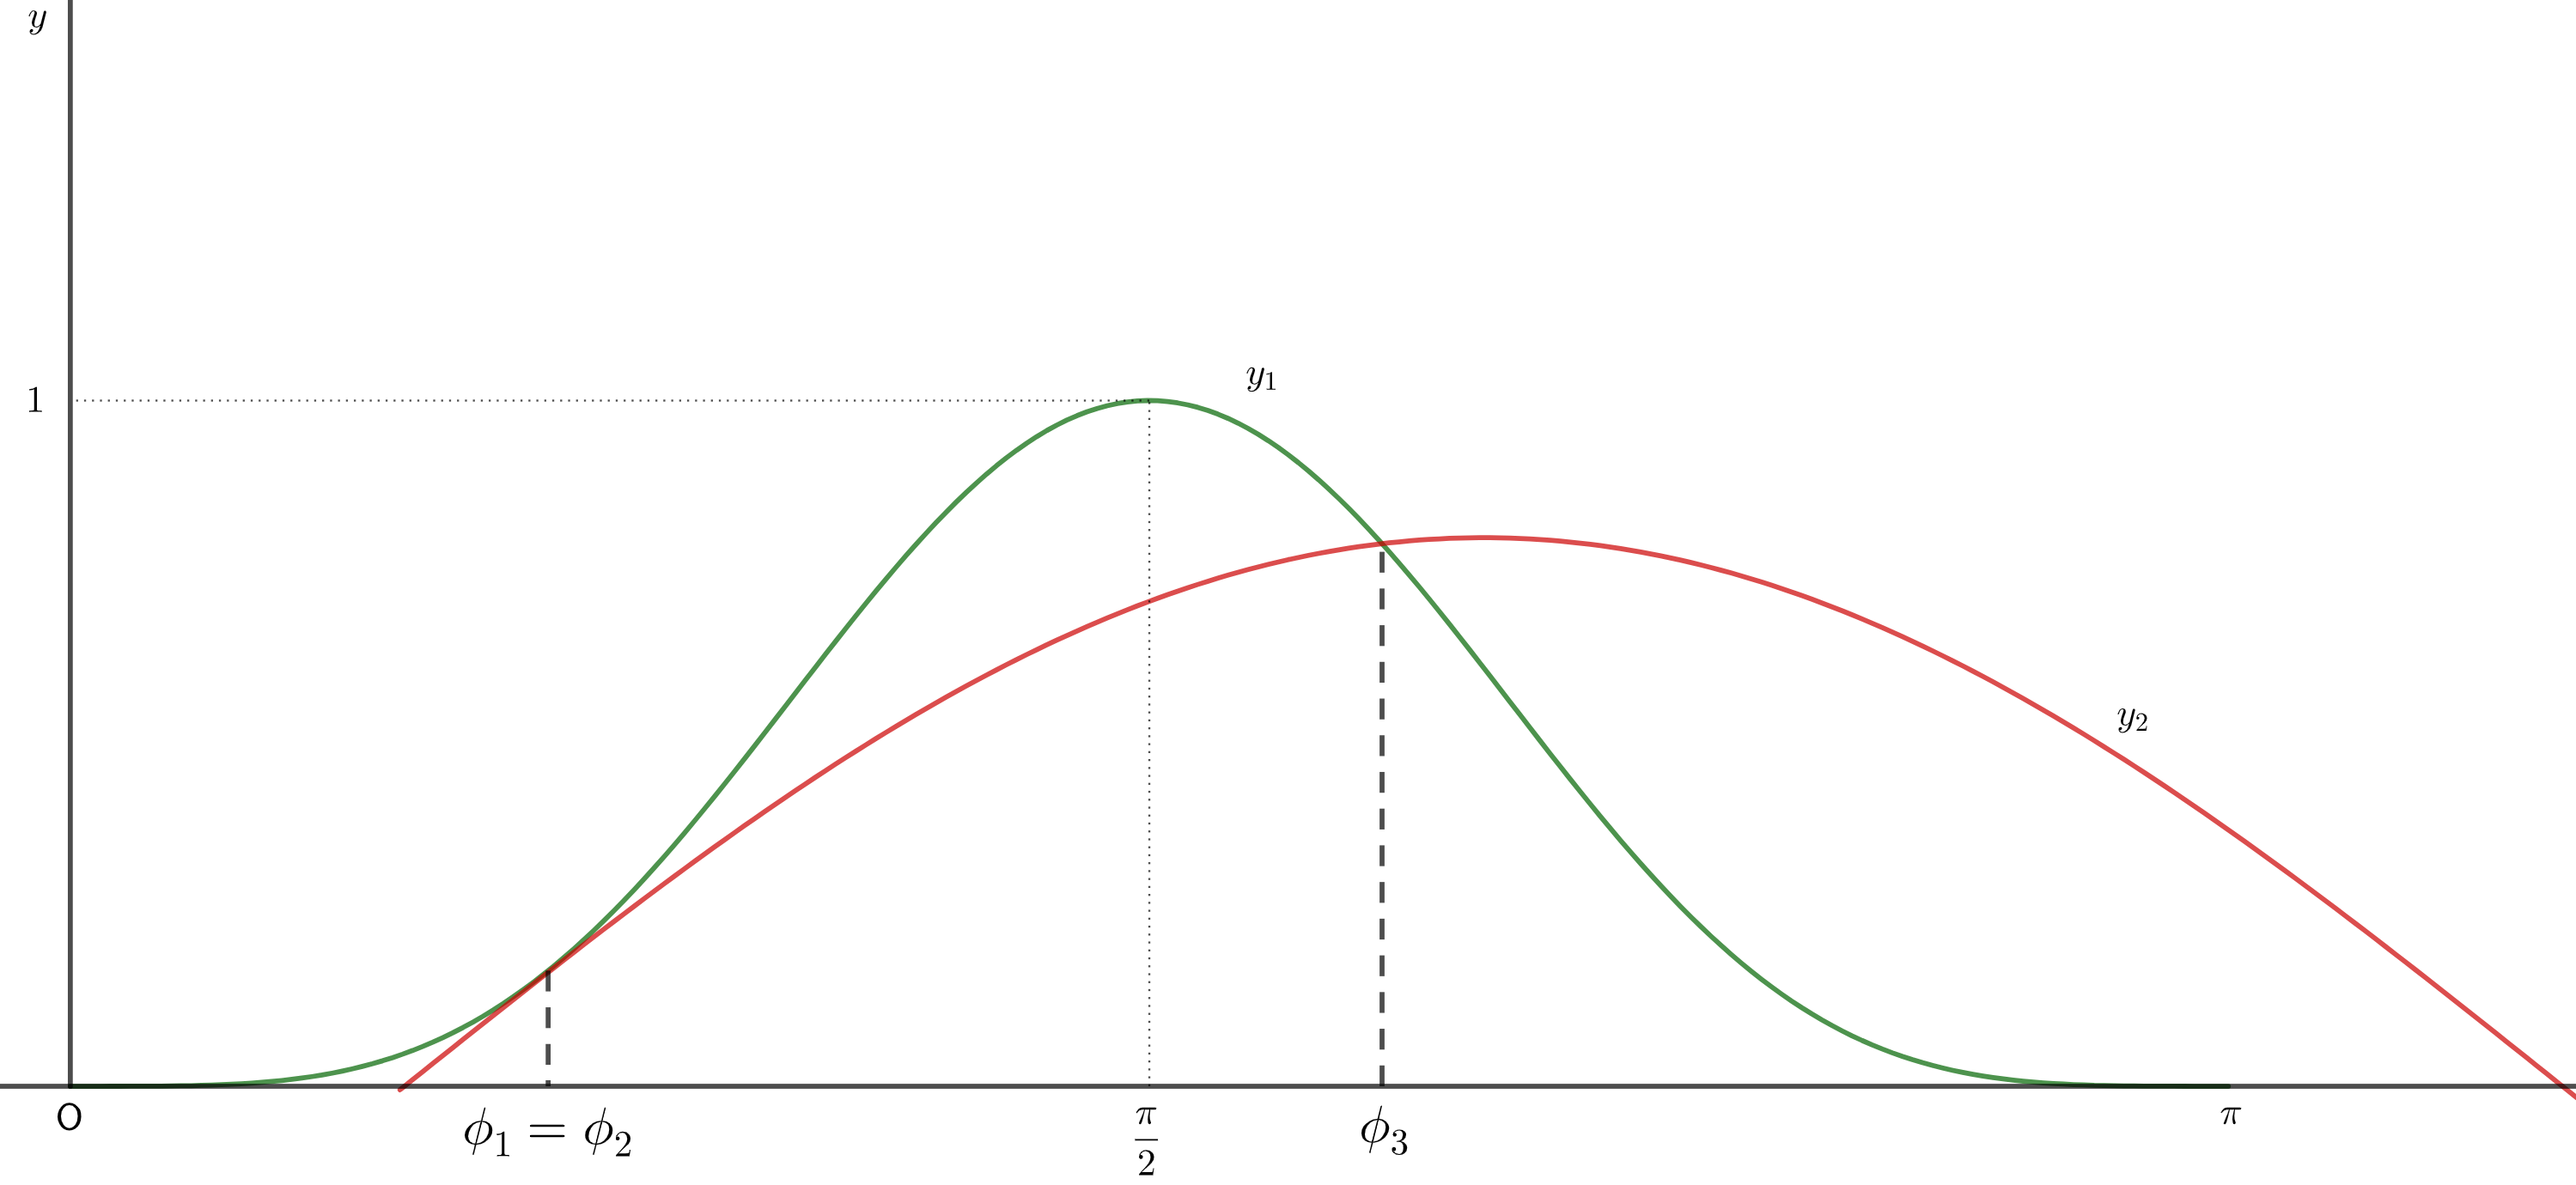
\includegraphics[scale=0.1]{images/minuscula_varia_primer_caso.png}
%	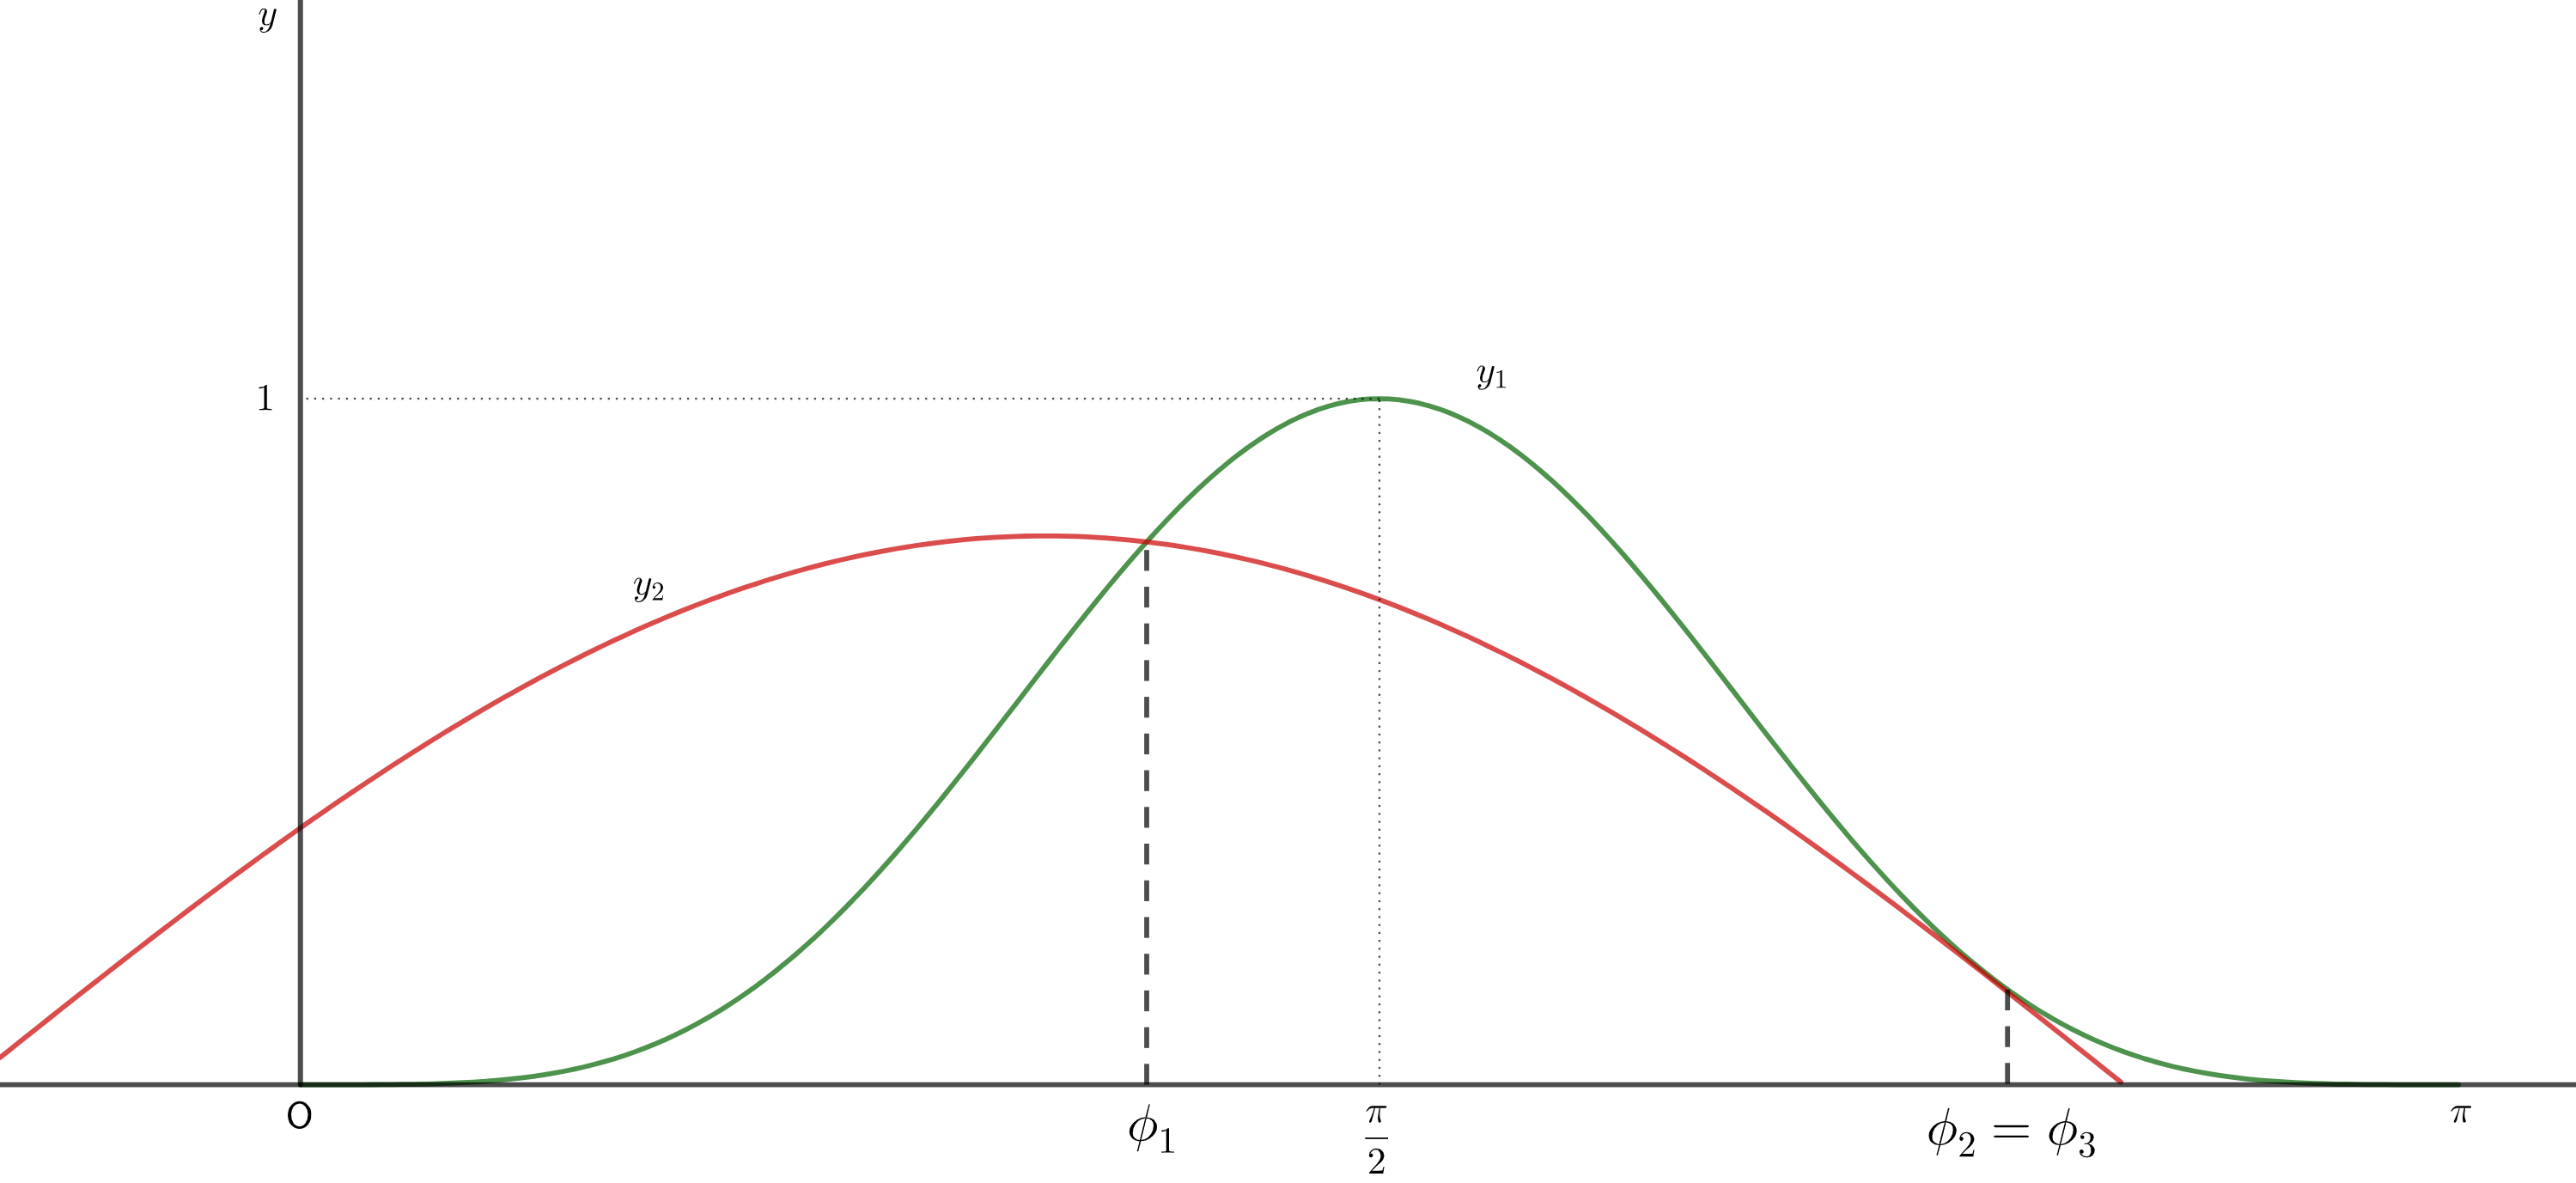
\includegraphics[scale=0.1]{images/minuscula_varia_segundo_caso.png}
%}
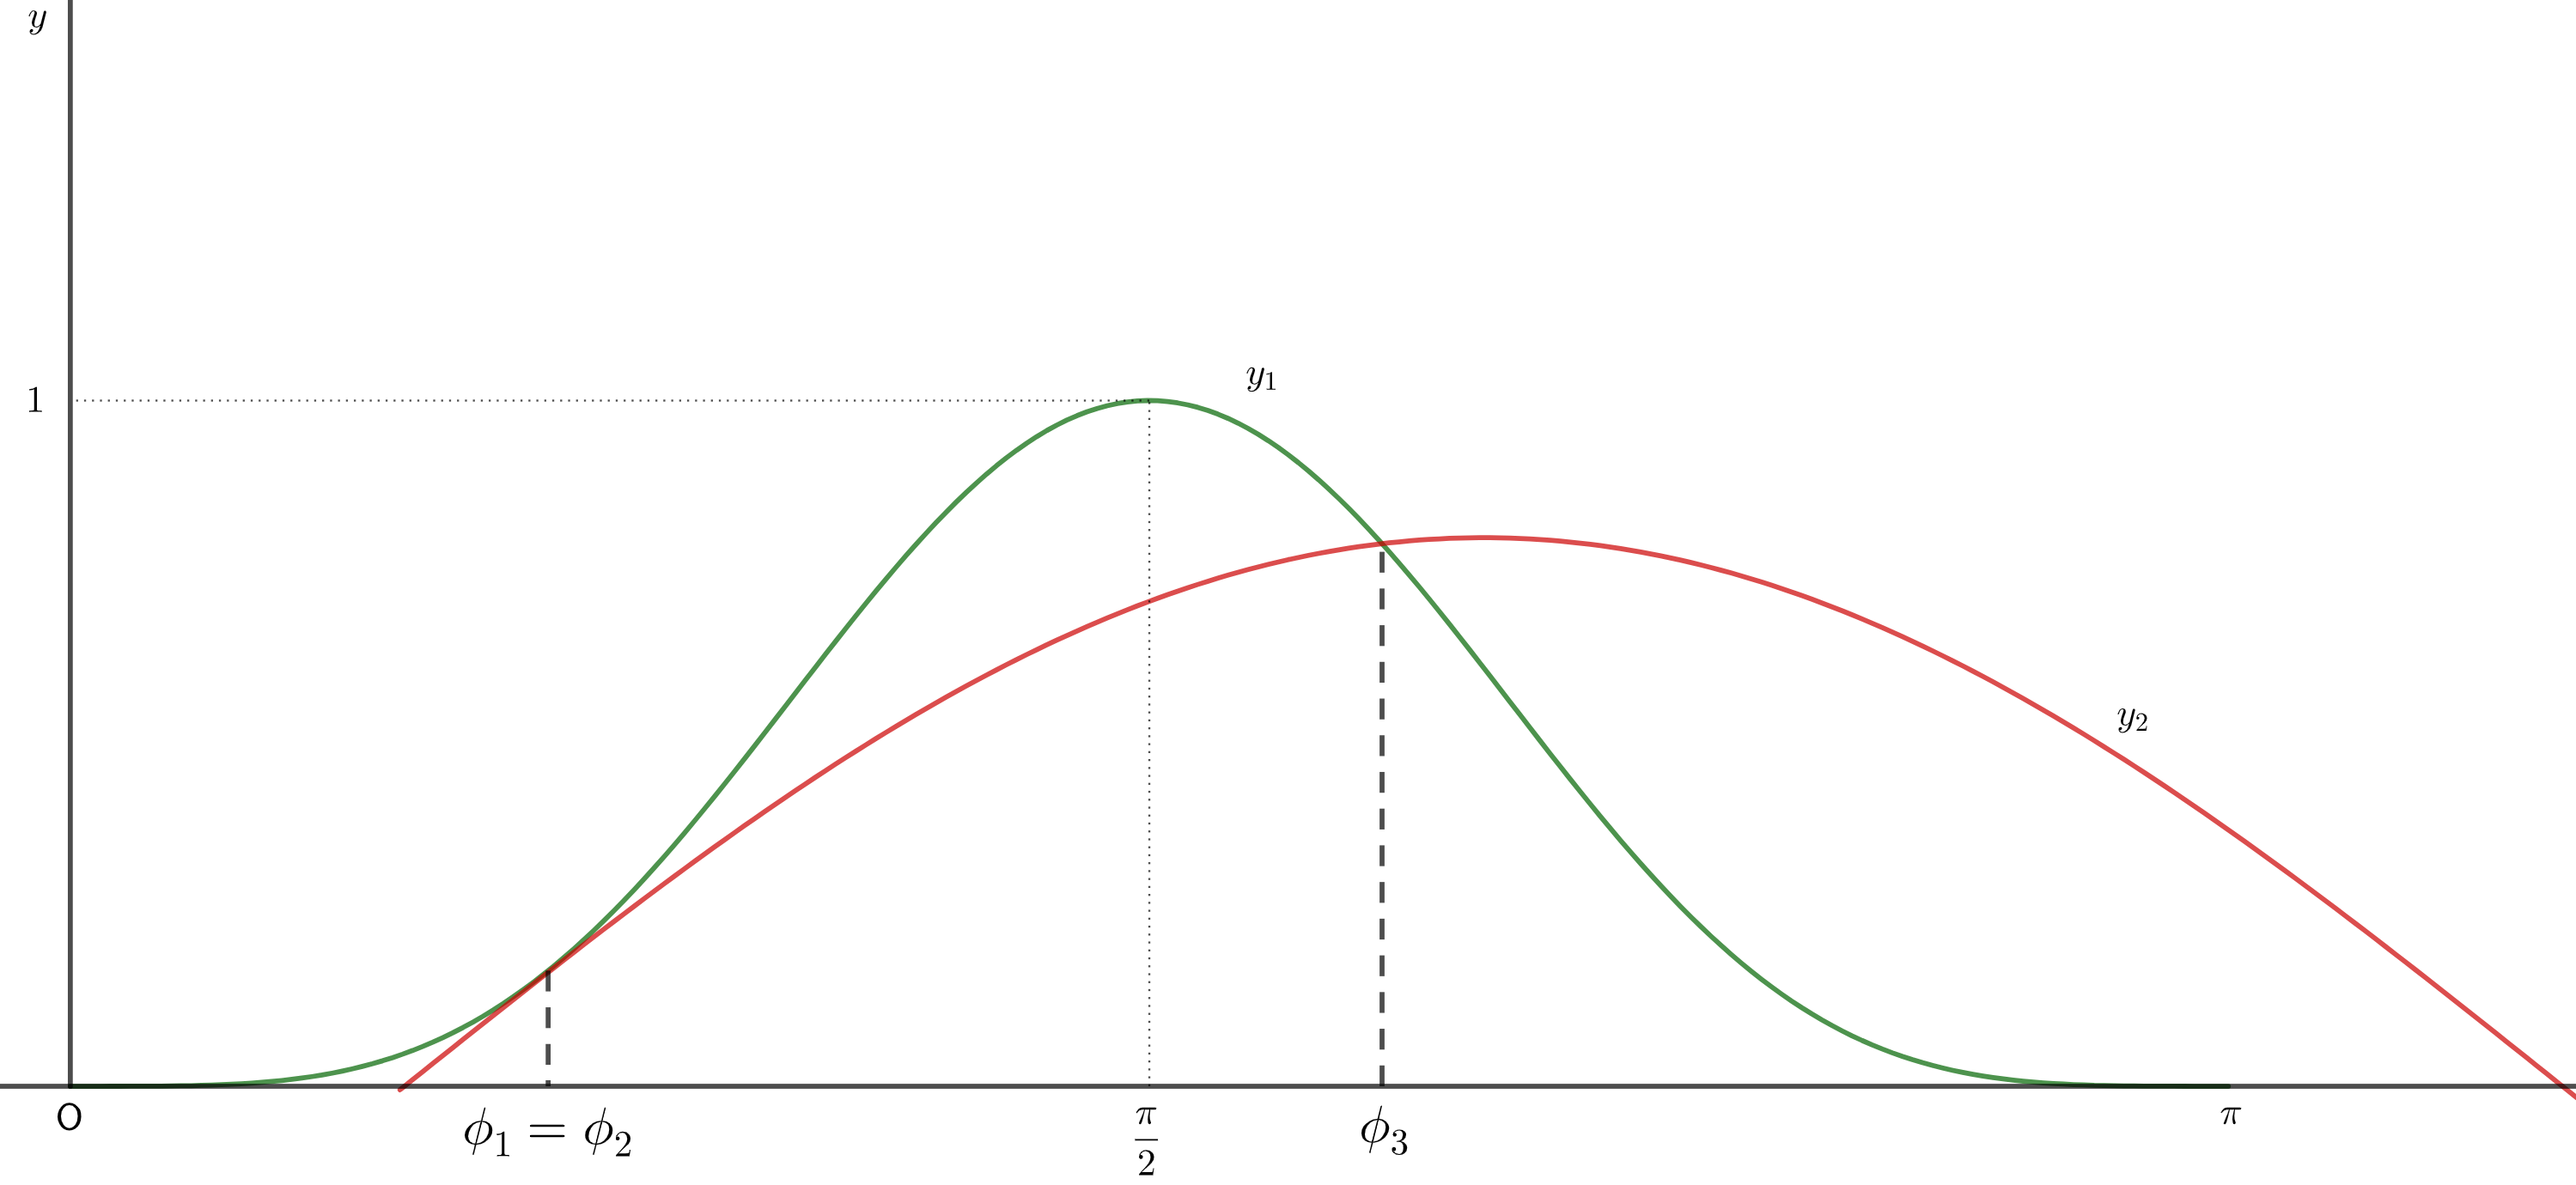
\includegraphics[scale=0.115]{images/minuscula_varia_primer_caso.png}
\caption{Variación de $m$ en la figura \ref{fig:phi_solution_m_negative_M_near_1} hasta obtener una solución doble.}
\label{fig:minuscula_varia_primer_caso}
\end{figure}

\begin{figure}[H]
\centering
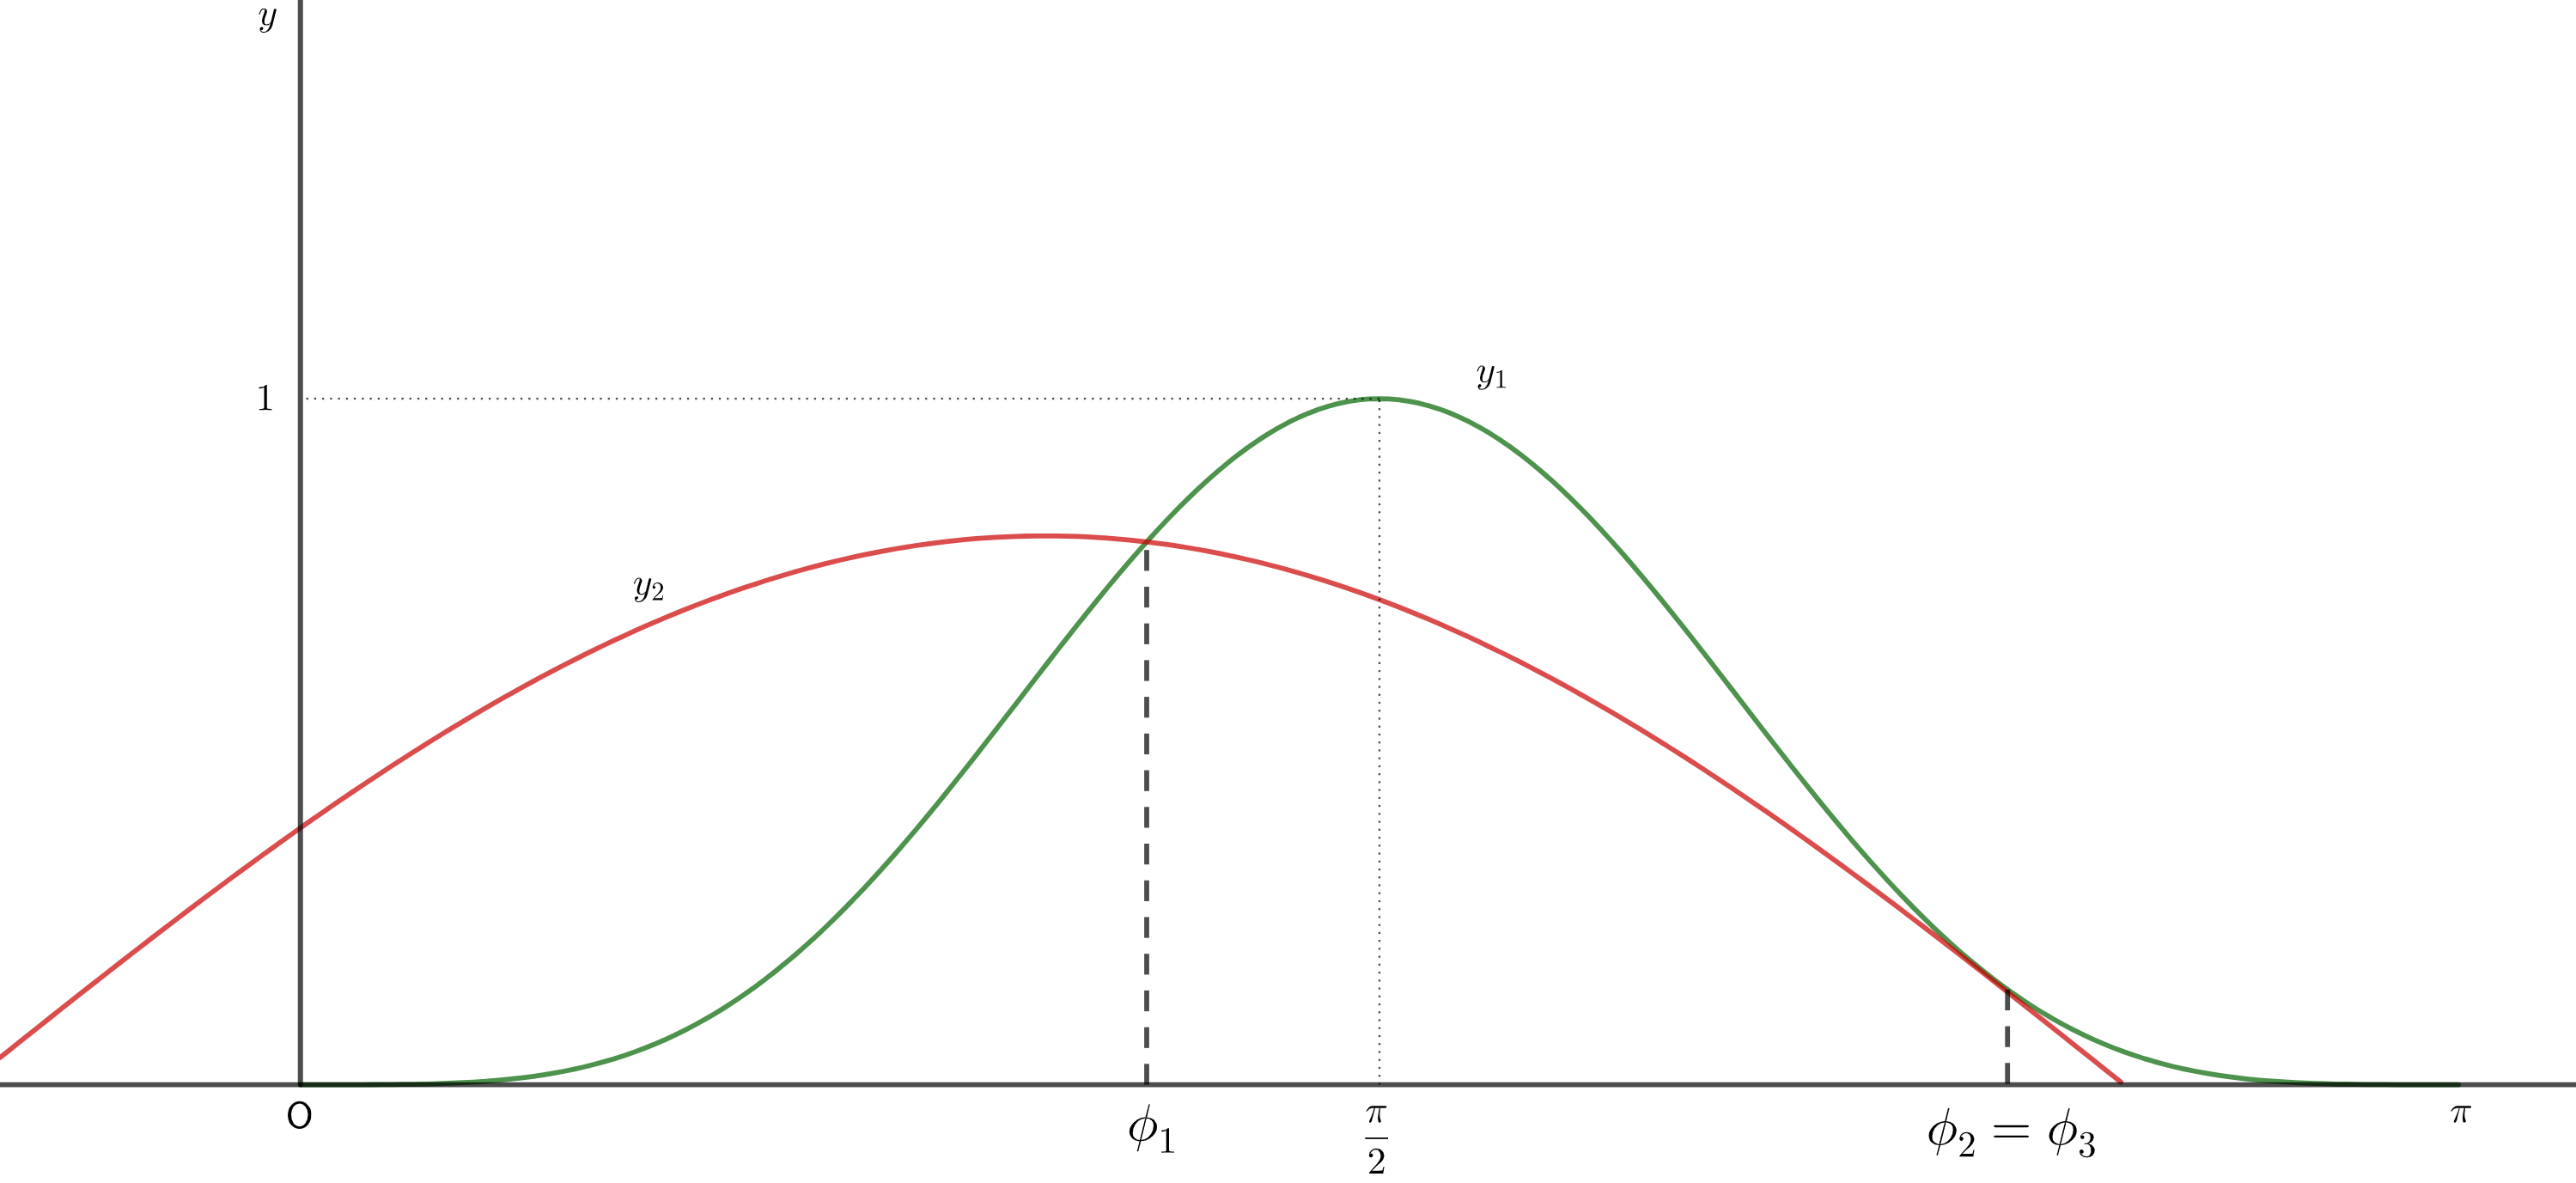
\includegraphics[scale=0.115]{images/minuscula_varia_segundo_caso.png}
\caption{Variación de $m$ en la figura \ref{fig:phi_solution_m_positive_M_near_1} hasta obtener una solución doble.}
\label{fig:minuscula_varia_segundo_caso}
\end{figure}

Veamos ahora el otro caso; fijamos $m$ y vamos aumentando $M$ empezando desde un valor pequeño. Conforme $M$ aumente, la amplitud de $y_2$ aumentará, dejando fijo, en el primer caso (figura \ref{fig:phi_solution_m_negative_M_near_1}), $\phi_1$ y llegando a un punto donde $\phi_2$ y $\phi_3$ serán iguales. Funcionará análogamente con el segundo caso.

\begin{figure}[H]
\centering
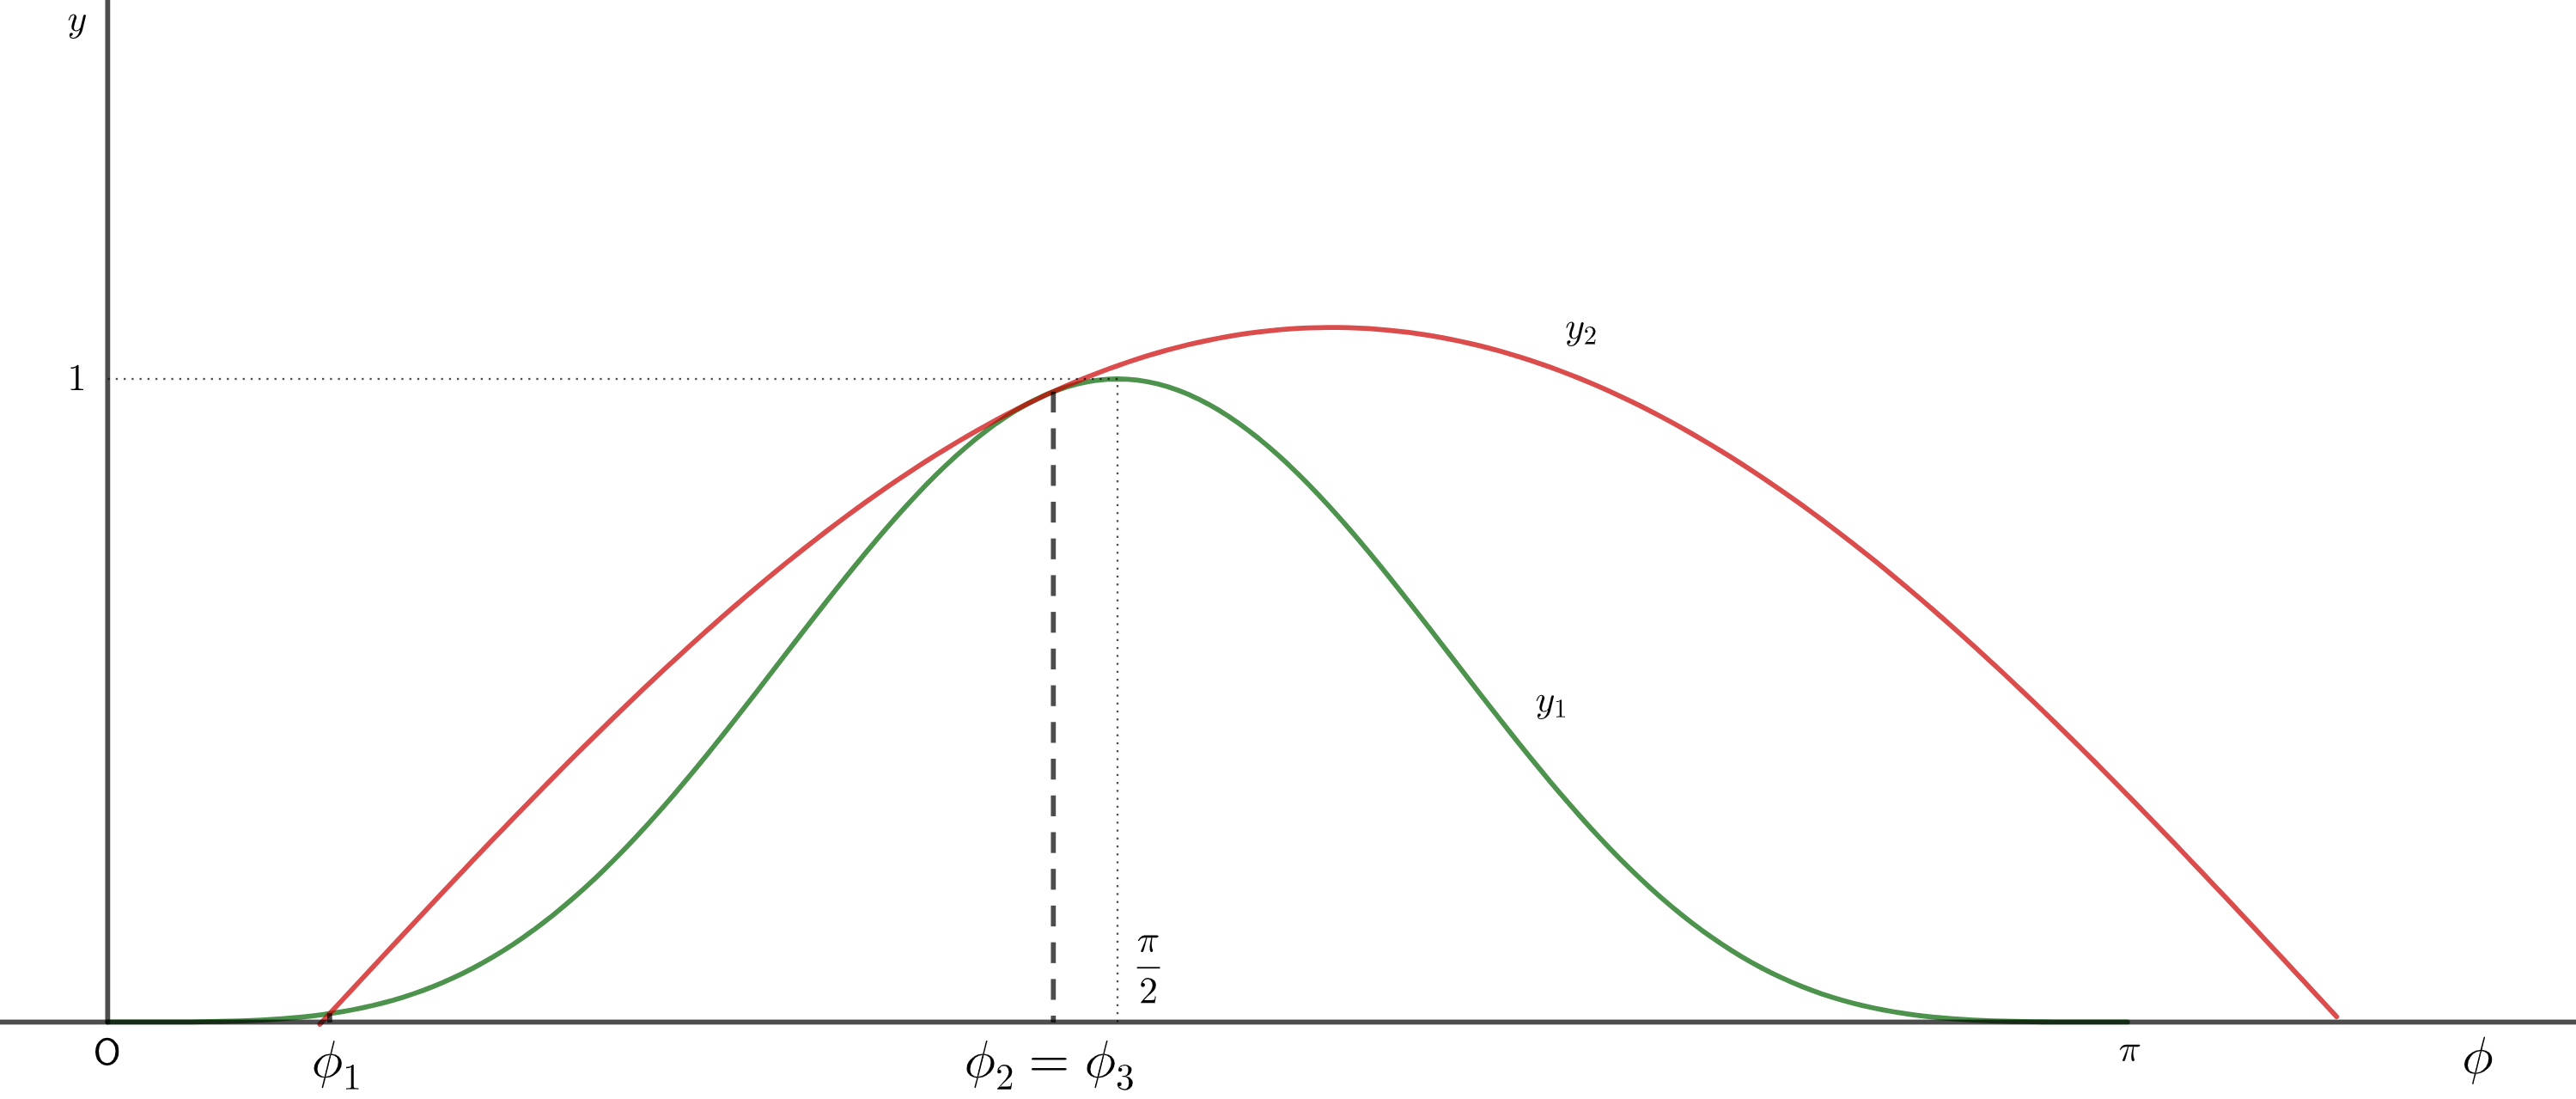
\includegraphics[scale=0.115]{images/mayuscula_varia_primer_caso.png}
\caption{Variación de $M$ en la figura \ref{fig:phi_solution_m_negative_M_near_1} hasta obtener una solución doble.}
\label{fig:mayuscula_varia_primer_caso}
\end{figure}

\begin{figure}[H]
\centering
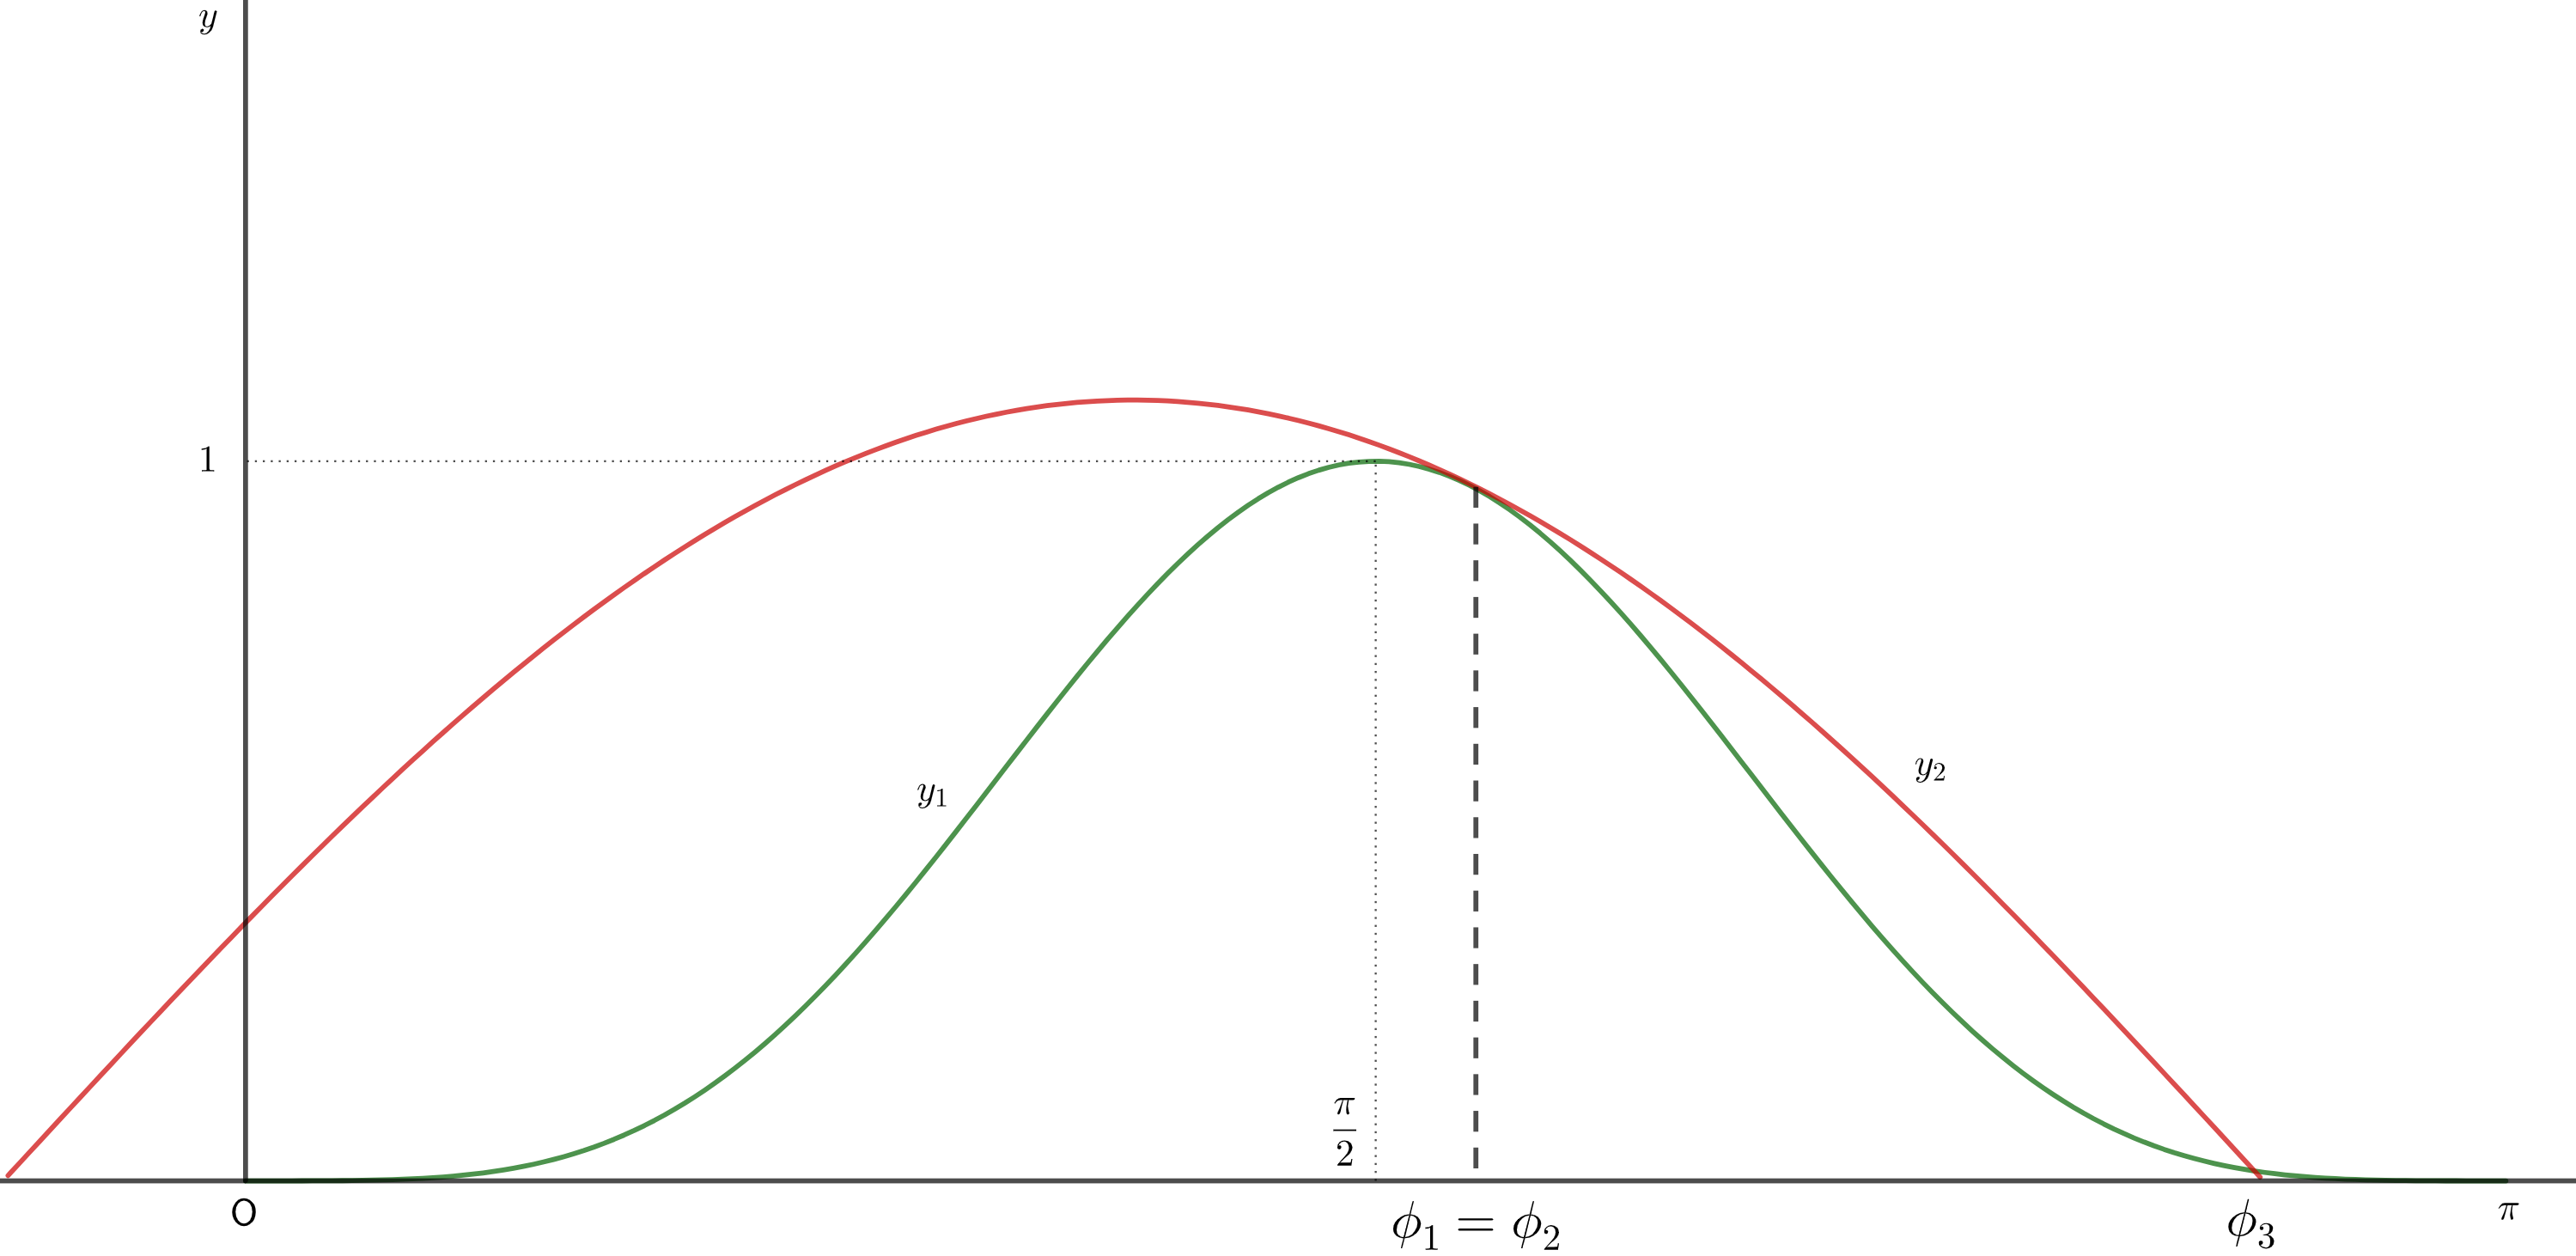
\includegraphics[scale=0.115]{images/mayuscula_varia_segundo_caso.png}
\caption{Variación de $M$ en la figura \ref{fig:phi_solution_m_positive_M_near_1} hasta obtener una solución doble.}
\label{fig:mayuscula_varia_segundo_caso}
\end{figure}

Las condiciones en las que la ecuación \eqref{eq:phi_solution} tendrá una solución doble son:
\begin{align}
\left\{
\begin{array}{l}
	\sin^4{\phi}=M\sin{(\phi+m)}\\
	4\sin^3{\phi}\cos{\phi}=M\cos{(\phi+m)}
\end{array}
\right.
\label{eq:condicion_raiz_doble}
\end{align}

Con el fin de encontrar las condiciones a las que esté sujeto $m$ para que la raíz sea doble, dividamos las dos ecuaciones superiores y resolvamos para la $\tan{\phi}$.
\begin{align}
\def\arraystretch{2}
\begin{array}{ll}
  & \ddfrac{\sin^4{\phi}}{4\sin^3{\phi}\cos{\phi}}=\ddfrac{M\sin{(\phi+m)}}{M\cos{(\phi+m)}}\Longrightarrow \ddfrac{1}{4}\tan{\phi}=\tan{(\phi+m)}\\
\Longrightarrow & \ddfrac{1}{4}\tan{\phi}=\ddfrac{\tan{m}+\tan{\phi}}{1-\tan{m}\tan{\phi}} \Longrightarrow \tan{\phi}-(\tan{\phi})^2\tan{m}=4\tan{m}+4\tan{\phi}\\
\Longrightarrow & \tan^2{\phi}\tan{m}+3\tan{\phi}+4\tan{m}=0 \Longrightarrow \tan{\phi}=\ddfrac{-3\pm\sqrt{9-16\tan^2{m}}}{2\tan{m}}
\end{array}
\label{eq:tan_phi}
\end{align}

Así, para que $\tan{\phi}$ tenga soluciones reales $m$ ha de estar sujeto a la condición:
\[
9-\tan^2{m}\geq0,
\]
\noindent y resolviendo esta inecuación para $m$ obtendremos:
\begin{align}
\left\{
\begin{array}{l}
	0 \leq m \leq 36º52'\\
	323º8' \leq m \leq 360º
\end{array}
\right.
\label{eq:m_condition}
\end{align}

El primer rango de valores pertenecerá al segundo caso comentado, representado en la figura \ref{fig:phi_solution_m_positive_M_near_1}, y viceversa.\\

Utilizando este rango de valores, para cada $m$ habrá dos soluciones de \eqref{eq:tan_phi} en el intervalo $(0,\pi)$. Si tomamos $m$ entre $323º8'$ y $360º$, la tangente de $m$ será negativa y $\tan{\phi}$ será positiva independientemente de qué signo tomemos antes de la raíz; además, $\tan{\phi}$ será menor cuando cojamos el signo negativo. De tal manera, si tomamos el radical positivo estaremos en el caso $\phi_1=\phi_2$ (figura \ref{fig:minuscula_varia_primer_caso}) y si lo tomamos negativo estaremos en el caso $\phi_2=\phi_3$ (figura \ref{fig:mayuscula_varia_primer_caso}). Por último, si tomamos $m$ como un valor límite del intervalo estaremos ante el caso $9-\tan^2{m}=0$, por lo que $\phi_1=\phi_2=\phi_3$. Si tomamos el caso $0 \leq m \leq 36º52'$ tendremos que $\tan{m}>0$ y la discusión será análoga a la anterior.\\

Los valores límite de $\phi$ definidos por \eqref{eq:tan_phi} según el rango de valores para $m$ serán:
\begin{align}
\phi=\arctan{(\ddfrac{-3}{2\tan{m}})} \Longrightarrow
\left\{
\begin{array}{l}
	\phi=116º34'\\
	\phi=63º26'
\end{array}
\right.
\end{align}

Utilizando estos valores de $\phi$ podemos obtener un valor para $M$ mediante las ecuaciones \eqref{eq:condicion_raiz_doble}, $M=1.431$, y dicho valor se corresponderá con el máximo $M$ para el cuál \eqref{eq:phi_solution} tiene tres soluciones en el intervalo $(0,\pi)$.\\

Supongamos que $m$ toma el valor límite $323º8'$ y va aumentando hasta su límite superior, $360º$. Como hemos visto anteriormente, comenzaremos teniendo una raíz doble y los dos valores de $\phi$ se corresponderán con $63º26'$, y conforme $m$ aumente, uno irá hacia $0º$ y otro hacia $90º$. Respecto a los dos valores correspondientes a $M$, comenzarán en el límite, $M=1.431$, e irán decreciendo, uno de ellos hasta $0$ y el otro hasta la unidad. Notar que para cada $m$ que tomemos en los intervalos definidos en \eqref{eq:m_condition} existirán dos límites de $M$ de manera que \eqref{eq:phi_solution} tenga tres soluciones reales; por tanto, estos límites han de ser tenidos en cuenta con el fin de reducir el trabajo lo máximo posible.\\













\newpage

\begin{thebibliography}{99}
\bibitem{moulton} \textsc{Forest Ray Moulton}, \textsc{An Introduction to Celestial Mechanics}, \textit{second edition}.

\bibitem{ortega} \textsc{R. Ortega, A.J. Ureña}, \textsc{Introducción a la Mecánica Celeste}.

\bibitem{right_ascension_declination} \textsc{Sky \& Telescope}, \textsc{Right Ascension and Declination: Celestial Coordinates For Beginners}, \url{https://skyandtelescope.org/astronomy-resources/right-ascension-declination-celestial-coordinates/}

\bibitem{ASA} \textsc{Solution of triangles}, \url{https://en.wikipedia.org/wiki/Solution_of_triangles#A_side_and_two_adjacent_angles_given_(ASA)}

\bibitem{unitary} \textsc{Notes on Coordinate Systems and Unit Vectors}, \url{http://www.physics.purdue.edu/~jones105/phys310/coordinates.pdf}

\end{thebibliography}

\end{document}


